\documentclass[12pt, oneside]{amsart}  	% use "amsart" instead of "article" for AMSLaTeX format
\usepackage{geometry}                		% See geometry.pdf to learn the layout options. There are lots.
\geometry{letterpaper}                   		% ... or a4paper or a5paper or ...
%\geometry{landscape}                		% Activate for for rotated page geometry
%\usepackage[parfill]{parskip}    		% Activate to begin paragraphs with an empty line rather than an indent
\usepackage{graphicx}				% Use pdf, png, jpg, or eps§ with pdflatex; use eps in DVI mode
								% TeX will automatically convert eps --> pdf in pdflatex
\usepackage{pgfplots}
\usepackage{amsmath}
\usepackage{mathtools}
\usepackage{graphicx}
\usepackage{amssymb}
\usepackage{amsthm}
\usepackage{enumerate}
\usepackage{epstopdf}
\newtheorem{prob}{Problem}
\newtheorem{definition}{Definition}
\newtheorem{remark}{Remark}
\newtheorem{theorem}{Theorem}
\newtheorem{proposition}{Proposition}
\newtheorem{lemma}{Lemma}
%%%%% Version 2

\DeclareGraphicsRule{.tif}{png}{.png}{`convert #1 `dirname #1`/`basename #1 .tif`.png}
\newcommand\F{\mathbb{F}} \newcommand\E{\mathbb{E}} \newcommand\R{\mathbb{R}}
\newcommand\Z{\mathbb{Z}} \newcommand\N{\mathbb{N}} \newcommand\C{\mathbb{C}}
\newcommand\Q{\mathbb{Q}} \newcommand\eps{\varepsilon}
\newcommand\cM{\mathcal{M}}	\newcommand\cA{\mathcal{A}}
\newcommand\cC{\mathcal{C}}



% Version 2
%%%%%%%%%%%%%%%%%%%%%%%%%%%%%%%%%%%%%%%%%%%%
\usepackage{pgf,tikz}
\usepackage{mathrsfs}
\newtheorem{exercise}{Exercise}
\newtheorem{example}{Example}
%\usepackage[above,below,verbose,section]{placeins}
%\usetikzlibrary[patterns]
\usepackage[unicode=true]{hyperref}
\hypersetup{colorlinks = false,pdftex}
%\usepackage{fullpage}
\usepackage{amsmath, amsthm}
\usepackage[bitstream-charter]{mathdesign}
\usepackage{eucal}
\usepackage[utf8]{inputenc}
\usepackage{amsaddr}
\usepackage[above,below,verbose,section]{placeins}
%\usepackage[utf8]{inputenc}
%\usepackage[bitstream-charter]{mathdesign}
%\usepackage{eucal}
%\geometry{verbose,tmargin=3cm,bmargin=3cm,lmargin=2.54cm,rmargin=2.54cm,headheight=2.54cm}
%%%%%%%%%%%%%%%%%%%%%%%%%%%%%%%%%%%%%%%%%%%%


\usetikzlibrary{arrows}

\title{Homogenization of Hamilton-Jacobi equations\\
Notes and remarks}
\author{Son Nguyen Thai Tu}
\address[S. Tu]{Department of Mathematics, University of Wisconsin at Madison}
\email[S.~Tu]{thaison@math.wisc.edu}

\author{Son Phung Truong Van}
\address[S. Van]{Department of Mathematical Sciences, Carnegie Mellon University}
\email[S.~Van]{sonv@andrew.cmu.edu}

\date{}							% Activate to display a given date or no date







\begin{document}
\maketitle
%\emph{Disclaimer.} These things take some times to digest and understand the \\
%tricks/theorems/techniques. Any errors were mine, due to lack of understanding or typos.

%---------------------------------------------------------------------------------
\begin{abstract}
These notes contain the essential materials and some further remarks of the summer course "Homogenization of Hamilton-Jacobi equations" taught by Prof. Hung V. Tran\footnotemark at University of Science, Ho Chi Minh City, Viet Nam from July $6^{\text{th}}$ to July $14^{\text{th}}$, 2015.
\end{abstract}
\footnotetext{Department of Mathematics, University of Wisconsin at Madison}


%\tableofcontents




\newpage



\paragraph{\textbf{Notations:}}
\begin{itemize}
	\item $\mathbb{T}^n=\R^n/\Z^n$ is the $n$-dimensional donut (torus).
	\item w.r.t: with respect to
\end{itemize}
%%%%%%%%%

\vspace*{0.5cm}

\vspace*{0.5cm}
\section*{{\LARGE Lecture 1}}
%\addcontentsline{toc}{section}{Lecture 1}
\vspace*{0.5cm}

%For personal reasons, I didn't attend the first lecture.
Clear contest : $\varepsilon>0$ : scale of the equation, $\varepsilon \ll 1$ : $\varepsilon$ is very small.\\

\paragraph{\textbf{Equation of interest.}} Following the Hamilton-Jacobi equation
\begin{equation}
u_t^{\varepsilon} (x,t) + H\left(\frac{x}{\varepsilon},Du^\varepsilon(x,t)\right) = 0\qquad\text{in}\;\mathbb{R}^n\times (0,\infty) \tag{I} \label{eq}
\end{equation}

where

\begin{itemize}
\item $u^\varepsilon(x,t): \mathbb{R}^n\times[0,\infty)\longrightarrow\mathbb{R}$,\\ $x$ is the location variable (spatial) and $t$ is the time variable.
\item $u_t^\varepsilon(x,t) = \frac{\partial}{\partial t}u^\varepsilon(x,t)$.
\item $Du^\varepsilon(x,t) = \nabla_x(u^\varepsilon)(x,t) = \left(\frac{\partial u^\varepsilon}{\partial x_1},\ldots, \frac{\partial u^\varepsilon}{\partial x_n}\right)$.
\item $H$ is the Hamiltonian (total energy)
\begin{align*}
H: \mathbb{R}^n\times \mathbb{R}^n &\longrightarrow \mathbb{R}\\
(y,p)&\longmapsto H(y,p) \in \mathbb{R}.
\end{align*}
\end{itemize}


\begin{example}[Classical mechanics]
\begin{equation*}
H(y,p) = \frac{1}{2}|p|^2 + V(y)
\end{equation*}
where the first term is the kinetic energy and the second one is the potential energy.
\end{example}

\paragraph{\textbf{Question.}}
We want to understand (\ref{eq}) as $\varepsilon\longrightarrow 0$. Is there some $u$ such that $u_\varepsilon\longrightarrow u$ and is $u$ solve something simpler? This is one of the key questions in homogenization theory.\\



\paragraph{\textbf{Assumptions.}} The following assumptions are extremely important:
\begin{itemize}
\item[(H1)] (coercivity)
\begin{equation*}
\lim_{|p|\longrightarrow\infty} H(y,p) = \infty \qquad\text{uniformly in}\;y,
\end{equation*}
\item[(H2)] (periodicity)
\begin{equation*}
H(y+k,p) = H(y,p) \qquad\forall\;k\in \mathbb{Z}^n.
\end{equation*}
\end{itemize}


\paragraph{\textbf{Formal Analysis.}} (not rigorous) Consider the equation
\begin{equation}\label{II}
u_t^{\varepsilon} (x,t) + H\left(\frac{x}{\varepsilon},Du^\varepsilon(x,t)\right) = 0 \tag{$I$}
\end{equation}
where $t$ is time variable, $x$ is spatial variable (slow variable) and $y = \frac{x}{\varepsilon}$ is the fast oscillatory variable. There are several ways to begin our analysis:
\begin{itemize}
\item Numerical analysis: plot $u^\varepsilon$.
\item Guessing: some asymptotic expansion w.r.t $\varepsilon$.
\end{itemize}
We consider some ansatzs\footnote{The word \textit{Ansatz} in German is some thing like the word \textit{formulation} in English.}

\begin{itemize}
\item[(1)] $u^\varepsilon(x,t) = u(x,t)+\varepsilon u^1\left(x,\frac{x}{\varepsilon},t\right) + \varepsilon^2 u^2\left(x,\frac{x}{\varepsilon},t\right) + \ldots$ \vspace*{0.5cm}
\item[(2)] $u^\varepsilon(x,t) = u\left(x,\frac{x}{\varepsilon},t\right) + \varepsilon u^1\left(x,\frac{x}{\varepsilon},t\right) + \ldots$.
\vspace*{0.5cm}
\item[(3)] $u^\varepsilon(x,t) = u\left(x,t\right) + \varepsilon^5 u^1\left(\frac{x}{\varepsilon},t\right) + \ldots$.
\vspace*{0.5cm}
\item[(4)] $u^\varepsilon(x,t) = u(x,t)+\varepsilon u^1\left(\frac{x}{\varepsilon},t\right) + \varepsilon^2 u^2\left(\frac{x}{\varepsilon},t\right) + \ldots$
\end{itemize}
Now using (4), we have
\begin{align*}
u^\varepsilon(x,t) &= u(x,t)+\varepsilon u^1\left(\frac{x}{\varepsilon},t\right) + \varepsilon^2 u^2\left(\frac{x}{\varepsilon},t\right) + \ldots \\
Du^\varepsilon(x,t) &= Du(x,t)+Du^1\left(\frac{x}{\varepsilon},t\right) + \varepsilon Du^2\left(\frac{x}{\varepsilon},t\right) + \ldots
\end{align*}
Plugging these into (\ref{II}) we have
\begin{equation*}
\left[u_t^\varepsilon(x,t) + \varepsilon u^1_t\left(\frac{x}{\varepsilon},t\right) + \ldots \right] + H\left( \frac{x}{\varepsilon}, Du(x,t)+Du^1\left(\frac{x}{\varepsilon},t\right) + \varepsilon Du^2\left(\frac{x}{\varepsilon},t\right) + \ldots\right)=0.
\end{equation*}
Denote $y = \frac{x}{\varepsilon}$, we obtain
\begin{equation*}
\left[u_t^\varepsilon(x,t) + \varepsilon u^1_t\left(y,t\right) + \ldots \right] + H\left( y, Du(x,t)+Du^1\left(y,t\right) + \varepsilon Du^2\left(y,t\right) + \ldots\right)=0.
\end{equation*}
{ \textbf{We will assume a ``big lie"}:} $x$ and $y$ are independent. Matching asymptotic expansion zero-order term $O(1)$, we get
\begin{equation*}
u_t(x,t) + H\Big(y,Du(x,t) + Du^1(y,t)\Big) = 0.
\end{equation*}
Now, fix $(x,t)\in \mathbb{R}^n\times(0,\infty)$, since $u_t(x,t)$ is a constant w.r.t $y$,
$$H(y,Du(x,t) + Du^1(y,t))$$
is expected to be a constant w.r.t $y$, i.e.,
\begin{equation*}
H(y,Du(x,t)+ Du^1(y,t)) = C(p,t).
\end{equation*}
Let $p= Du(x,t) \in \mathbb{R}^n$, then
\begin{equation*}
H(y,p+Du^1(y,t)) = C(p,t).
\end{equation*}
Assume one more reduction $u^1(y,t) = u^1(y)$, we then have the following PDE
\begin{equation*}
H(y, p+Du^1(y)) = C(p).
\end{equation*}
This is called the cell (or ergodic) problem.

\begin{theorem}[Lions-Pappanicolau-Varadhan]\label{theorem1}
 Fix $p\in \mathbb{R}^n$, there exists a unique constant $C\in \mathbb{R}^n$ such that the cell problem
\begin{equation*}
H(y, p+Du^1(y)) = C(p) \qquad\text{in}\;\mathbb{R}^n
\end{equation*}
has a periodic solution $u^1$.
\end{theorem}
Define the effective Hamiltonian $\overline{H}(p) = C(p)$. We are back to our original question: consider
\begin{equation}\label{C_eps}
	\begin{cases}
		u^\eps_t + H(\frac{x}{\eps}, Du^\eps)=0\\
		u^\eps(x,0)=u_0(x)
	\end{cases}\tag{$C_\eps$}.
\end{equation}
Do the solutions $u^\eps$ of (\ref{C_eps}) converges to a solution $u$ of
\begin{equation} \label{HJ}
	\begin{cases}
		u_t + \overline{H}(Du)=0\\
		u(x,0)=u_0(x)
	\end{cases}?\tag{HJ}
\end{equation}
\begin{remark} This is a natural question  since from the Hamiltonian $H(\frac{x}{\eps}, Du^\eps)$ we derived the effective Hamiltonian $\overline{H}$ that is independent of $\eps$ so as we pass $\eps\to 0$, (\ref{C_eps}) should become (\ref{HJ}). The answer to this problem is ``yes'' and will be elaborated in lecture 3.
\end{remark}






\newpage


\section*{{\LARGE Lecture 2}}
\vspace*{0.5cm}

Before we prove theorem \ref{theorem1}, let's talk about viscosity solutions. \vspace*{0.5cm}

\paragraph{\textbf{Introduction to viscosity solutions.}}

Consider
\begin{itemize}
\item The static problem
\begin{equation}\label{S}
	u(y)+H(y,Du(y))=0 \tag{S}.
\end{equation}
\item The Cauchy problem
\begin{equation}\label{C}
\begin{cases}
u_t(x,t) + H(y,Du(x,t)) = 0 &\qquad\text{in}\;\mathbb{R}^n\times (0,\infty)\\
u(y,0)  = u_0(y) &\qquad\text{on}\;\mathbb{R}^n
\end{cases} \tag{$C$}.
\end{equation}
\end{itemize}



We then look into the static problem in $\R^n$. The idea here is that the problem
\begin{equation}\label{S_varepsilon}
	u^\eps + H(Du^\eps(y), y)=\eps\Delta u^\eps \text{ in } \R^n \tag{$S_\varepsilon$}
\end{equation}
has a smooth solution $u^\eps$. Assume further that $u^\eps \to u$ locally uniformly in $\mathbb{R}^n$. %%version 1.
Take a smooth function $\phi$ such that %version 1
\begin{equation*}
	\begin{cases}
		(u-\phi)(x_0)&=0\\
	\;\;	(u - \phi)(x) &< 0 \qquad\text{else where}
	\end{cases}.
\end{equation*}
That is, $u-\phi$ has a strict max at $x_0$.
\begin{exercise}\label{exercise1}
For $\eps>0$ small enough, $u^\eps -\phi$ has a max at $x_\eps$ near by $x_0$ and there is a subsequence $\eps_j\longrightarrow 0$ such that $x_{\eps_j}\longrightarrow x_0$. \footnote{Morever, if  $u_m$ is continuous and $\phi$ is smooth such that $u_m \longrightarrow u$ uniformly on a compact set $\overline{\Omega}\subset\mathbb{R}^n$, and assume $u - \phi$ has a strict (local) maximum over $\overline{\Omega}$ as $x_0$, $u_m - \phi$ has (local) maximum over $\overline{\Omega}$ at $x_m$. Then we must have $x_m\longrightarrow  x_0$ as $m\longrightarrow\infty$. We have the convegence of whole sequence here, while in case $u^{\varepsilon}\longrightarrow u$ uniformly as $\varepsilon\longrightarrow 0$ we only have the convergence of sub-sequence.}
\end{exercise}
\paragraph{\textbf{Play with $u^\varepsilon$.}} Since $u^\varepsilon -\phi$ has max at $x_\varepsilon$, we then have, of course by second derivative test,
\begin{equation}\label{reconsider.PDE}
\begin{cases}
	Du^\eps(x_\eps)=D\phi(x_\eps) &\;\Longrightarrow Du^\varepsilon(x_\varepsilon) = D\phi(x_\varepsilon) \\
	\Delta(u^\eps - \phi)(x_\eps)\le 0 &\Longleftrightarrow \Delta u^\eps(x_\eps)\le \Delta\phi(x_\eps)
\end{cases}.
\end{equation}
Reconsider the PDE,
\begin{equation*}
u^\eps(x_\eps) + H(x_\eps, Du^\eps(x_\eps))=\eps \Delta u^\eps(x_\eps).
\end{equation*}
From \eqref{reconsider.PDE}, we can see that
\begin{equation*}
u^\eps(x_\eps) + H(x_\eps, D\phi(x_\eps))\le \eps \Delta\phi(x_\eps).
\end{equation*}
Let $\eps_j\to 0$, we then have
\begin{equation*}
u(x_0)+ H(x_0, D\phi(x_0))\le 0.
\end{equation*}
Inspired by this derivation, we have the definition of viscosity solutions.

\begin{definition} [Definition of viscosity solution for the static equation] Assume $u$ is continuous on its domain
\begin{itemize}
\item (Subsolution) $u$ is called a viscosity subsolution if for all $\phi\in C^\infty(\R^n)$ such that $(u-\phi)(x_0)$ is a strict max then
$$u(x_0) + H(x_0, D\phi(x_0))\le 0.$$
\item (Supersolution) $u$ is called a viscosity supersolution if for all $\phi\in C^\infty(\R^n)$ such that $(u-\phi)(x_0)$ is a strict min then
$$u(x_0) + H(x_0, D\phi(x_0))\ge 0.$$
\item $u$ is called a viscosity solution if it is both a subsolution and a supersolution.
\end{itemize}
\end{definition}
% Version 1
%More about viscosity solutions can be found in Evans's book or last summer lecture notes.

\paragraph{\textbf{Geometric descriptions.}} Using the notions of sub-differential and super-differential, we will give a geometric descriptions for viscosity solution as the following


\begin{definition} Let $u$ be a real valued function defined on the open set $\Omega \subset \mathbb{R}^n$. For any $x\in \Omega$, the sets
\begin{align*}
D^-u(x) &= \left\lbrace p\in \mathbb{R}^n: \liminf_{y\longrightarrow x} \frac{u(y) - u(x) - \langle p,y-x\rangle}{\Vert y-x\Vert} \geq 0 \right\rbrace \\
D^+u(x) &= \left\lbrace p\in \mathbb{R}^n: \limsup_{y\longrightarrow x} \frac{u(y) - u(x) - \langle p,y-x\rangle}{\Vert y-x\Vert} \leq 0 \right\rbrace
\end{align*}
are called, respectively the \textbf{subdifferential} and \textbf{superdifferential} of $u$ at $x$.
\end{definition}
We can see that $p\in D^+u(x_0)$ if $u(x) \leq u(x_0) + p\cdot(x-x_0)$ for all $x\in B(x_0,r)$.



\begin{center}
\definecolor{ffqqqq}{rgb}{1.,0.,0.}
\definecolor{xdxdff}{rgb}{0.49019607843137253,0.49019607843137253,1.}
\begin{tikzpicture}[line cap=round,line join=round,>=triangle 45,x=1.0cm,y=1.0cm]
\clip(-3.,-0.5) rectangle (3.,4.);
\draw (-3.64,0.26)-- (-0.16479786329974505,2.70301323297317);
\draw (-0.16479786329974505,2.70301323297317)-- (1.16,-0.02);
\draw (-3.24,3.74)-- (3.64,1.42);
\draw (-0.34,3.38) node[anchor=north west] {$x_0$};
\draw [->,color=ffqqqq] (-0.16479786329974505,2.70301323297317) -- (0.8773922544615758,2.351577030472259);
\draw (0.42,3.16) node[anchor=north west] {$p$};
\draw (0.78,1.28) node[anchor=north west] {$u$};
\begin{scriptsize}
\draw [fill=xdxdff] (-0.16479786329974505,2.70301323297317) circle (1.5pt);
\draw [fill=xdxdff] (0.8773922544615759,2.351577030472259) circle (1.5pt);
\end{scriptsize}
\end{tikzpicture}
\end{center}

Similarly, $p\in D^-u(x)$ if $u(x) \geq u(x_0) + p\cdot(x-x_0)$ for all $x\in  B(x_0,r)$.

\begin{center}
\definecolor{ffqqqq}{rgb}{1.,0.,0.}
\definecolor{qqqqff}{rgb}{0.,0.,1.}
\definecolor{xdxdff}{rgb}{0.49019607843137253,0.49019607843137253,1.}
\begin{tikzpicture}[line cap=round,line join=round,>=triangle 45,x=1.0cm,y=1.0cm]
\clip(-3.,2.) rectangle (3.,5.);
\draw (-1.7,4.74)-- (-0.16479786329974505,2.70301323297317);
\draw (-0.16479786329974505,2.70301323297317)-- (3.22,4.56);
\draw (-3.24,3.74)-- (3.64,1.42);
\draw (-0.34,3.38) node[anchor=north west] {$x_0$};
\draw [->,color=ffqqqq] (-0.16479786329974505,2.70301323297317) -- (0.8773922544615758,2.351577030472259);
\draw (-0.08,2.52) node[anchor=north west] {$p$};
\draw (1.3,4.22) node[anchor=north west] {$u$};
\begin{scriptsize}
\draw [fill=xdxdff] (-0.16479786329974505,2.70301323297317) circle (1.5pt);
\draw [fill=qqqqff] (-1.7,4.74) circle (1.5pt);
\draw [fill=qqqqff] (3.22,4.56) circle (1.5pt);
\draw [fill=xdxdff] (0.8773922544615759,2.351577030472259) circle (1.5pt);
\end{scriptsize}
\end{tikzpicture}
\end{center}

From this, we can see that, up to a constant,
\begin{align*}
u-\phi \;\text{has a strict max at}\;x_0 &\Longleftrightarrow u\;\text{is touched from above by}\;\phi\;\text{at}\;x_0\\
&\Longleftrightarrow D\phi(x_0) \in D^+u(x_0),\\
u-\phi \;\text{has a strict min at}\;x_0 &\Longleftrightarrow u\;\text{is touched from below by}\;\phi\;\text{at}\;x_0\\
&\Longleftrightarrow D\phi(x_0) \in D^-u(x_0).
\end{align*}


\begin{tabular}{cc}
\begin{minipage}{0.5\columnwidth }
\definecolor{ffqqqq}{rgb}{1.,0.,0.}
\definecolor{qqqqff}{rgb}{0.,0.,1.}
\definecolor{xdxdff}{rgb}{0.49019607843137253,0.49019607843137253,1.}
\begin{tikzpicture}[line cap=round,line join=round,>=triangle 45,x=1.0cm,y=1.0cm]
\clip(-3.,-2.) rectangle (2.,1.);
\draw (-3.18,-1.68)-- (-0.24270245056616524,0.03702768294743963);
\draw (-0.24270245056616524,0.03702768294743963)-- (1.38,-2.9);
\draw (-0.38,0.78) node[anchor=north west] {$x_0$};
\draw [->,color=ffqqqq] (-0.24270245056616524,0.03702768294743963) -- (1.2369297074177488,-0.5317445671967946);
\draw (0.48,-0.18) node[anchor=north west] {$p$};
\draw (0.7,-1.22) node[anchor=north west] {$u$};
\draw [samples=50,rotate around={0.:(0.,0.)},xshift=0.cm,yshift=0.cm,domain=-3.0:3.0)] plot (\x,{(\x)^2/2/0.5});
\draw (-1.2,0.9) node[anchor=north west] {$\phi$};
\begin{scriptsize}
\draw [fill=xdxdff] (-0.24270245056616524,0.03702768294743963) circle (1.5pt);
\draw [fill=qqqqff] (-3.18,-1.68) circle (1.5pt);
\draw [fill=qqqqff] (1.38,-2.9) circle (1.5pt);
\draw [fill=xdxdff] (1.2369297074177488,-0.5317445671967946) circle (1.5pt);
\end{scriptsize}
\end{tikzpicture}
\end{minipage}
&
\begin{minipage}{0.5\columnwidth}
\definecolor{ffqqqq}{rgb}{1.,0.,0.}
\definecolor{qqqqff}{rgb}{0.,0.,1.}
\definecolor{xdxdff}{rgb}{0.49019607843137253,0.49019607843137253,1.}
\begin{tikzpicture}[line cap=round,line join=round,>=triangle 45,x=1.0cm,y=1.0cm]
\clip(-3.,-2.) rectangle (3.,3.);
\draw (-2.78,1.28)-- (-0.3564726235279836,-0.11375682894257588);
\draw (-0.3564726235279836,-0.11375682894257588)-- (1.8,3.26);
\draw (-0.46,-0.06) node[anchor=north west] {$x_0$};
\draw [->,color=ffqqqq] (-0.3564726235279836,-0.11375682894257588) -- (0.5190882602889397,0.525493504916839);
\draw (0.4,0.48) node[anchor=north west] {$p$};
\draw (-1.74,1.28) node[anchor=north west] {$u$};
\draw [samples=50,rotate around={-180.:(0.,0.)},xshift=0.cm,yshift=0.cm,domain=-3.0:3.0)] plot (\x,{(\x)^2/2/0.5});
\draw (-1.12,-0.1) node[anchor=north west] {$\phi$};
\begin{scriptsize}
\draw [fill=xdxdff] (-0.3564726235279836,-0.11375682894257588) circle (1.5pt);
\draw [fill=qqqqff] (-2.78,1.28) circle (1.5pt);
\draw [fill=qqqqff] (1.8,3.26) circle (1.5pt);
\draw [fill=xdxdff] (0.5190882602889397,0.525493504916839) circle (1.5pt);
\end{scriptsize}
\end{tikzpicture}
\end{minipage}
\end{tabular}

In fact, we have the following properties:
\begin{proposition}[Properties of sub-differentials and super-differentials]\quad \\
Let $f:\Omega\subset \mathbb{R}^n\longrightarrow \mathbb{R}$ and $x\in \Omega$ where $\Omega$ is open, then the following properties hold
\begin{itemize}
\item[(a)] $D^+f(x) = -D^-(-f)(x)$.
\item[(b)] $D^+f(x)$ and $D^-f(x)$ are convex (possibly empty).
\item[(c)] If $f\in C(\Omega)$, then $p\in D^+f(x)$ if and only if there is a function $\varphi \in C^1(\Omega)$ such that $\nabla \varphi (x) = p$ and $f - \varphi$ has a local maximum at $x$.
\item[(d)] If $f\in C(\Omega)$, then $p\in D^-f(x)$ if and only if there is a function $\varphi \in C^1(\Omega)$ such that $\nabla \varphi (x) = p$ and $f - \varphi$ has a local minimum at $x$.
\item[(e)] $D^+f(x)$ and $D^-f(x)$ are both nonempty if and only if $f$ is differentiable at $x$. In this case we have that $D^+f(x) = D^-f(x) = \{\nabla f(x) \}$.
\item[(f)] If $f\in C(\Omega)$, the sets of points where a one-sided differential exists
\begin{equation*}
\Omega^+ = \{x\in \Omega:D^+f(x)\neq \emptyset \} \qquad\qquad\Omega^- = \{x\in \Omega:D^-f(x)\neq \emptyset \}
\end{equation*}
are both non-empty. Indeed, they are dense in $\Omega$.
\end{itemize}
\end{proposition}



\begin{proof}\quad
\begin{itemize}
\item[(a)] It's clear since if $a_n \longrightarrow a$ then
\begin{equation*}
\limsup_{n\longrightarrow \infty}\;(-a_n) = -\liminf_{n\longrightarrow \infty} a_n
\end{equation*}
\item[(b)] It's also clearl from the definitions.
\item[(c)] Assume that $p\in D^+f(x)$, by definition, we can find $\delta > 0$ and a continuous increasing function $\sigma:[0,\infty)\longrightarrow \mathbb{R}$ with $\sigma(0) = 0$ such that
\begin{equation}\label{difff_ccc}
f(y) \leq f(x) + \langle p,y-x\rangle + \Vert y-x\Vert \sigma(\Vert y-x\Vert)
\end{equation}
for $\Vert y-x\Vert < \delta$. Define
\begin{equation*}
\rho(r) = \int_{0}^r \sigma(t)\;dt
\end{equation*}
then
\begin{equation*}
 \rho(0) = \rho'(0) = 0 \quad\text{and}\quad r\sigma(r)\leq \rho(2r)\leq r\sigma(2r)
\end{equation*}
Now for $y\in B(x,\delta)$ we set
\begin{equation*}
\varphi(y) = f(x) + \langle p,y-x\rangle + \rho(2\Vert y-x\Vert).
\end{equation*}
Since $f(x) = \varphi(x)$, clearly $\varphi$ is differentiable. Furthermore, because
\begin{equation*}
\sigma(r)\leq\frac{\rho(2\Vert y-x\Vert)}{\Vert y-x\Vert}  \leq \sigma(2\Vert y-x\Vert)
\end{equation*}
and $\sigma(r)\longrightarrow 0$ as $r\longrightarrow 0$, we conclude that $\nabla \varphi(x) = p$. Now for $y\in B(x,\delta)$, from \eqref{difff_ccc} we have
\begin{align*}
f(y) - f(x) &\leq \langle p,y-x\rangle + \Vert y-x\Vert\sigma(\Vert y-x\Vert)\\
 &\leq \langle p,y-x\rangle + \rho(2\Vert y-x\Vert) = \varphi(y) - \varphi(x).
\end{align*}
Therefore, $(f-\varphi)(y) \leq (f-\varphi)(x)$ for $y\in B(x,\delta)$, i.e, $f-\varphi$ has a local maximum at $x$.\\
For the converse, if $\varphi\in C^1(\Omega)$ such that $f-\varphi$ has a local maximum at $x$ and $f(x) = \varphi(x)$, $\nabla \varphi(x) = p$. Then, since $f(y) -f(x) \leq \varphi(y) - \varphi(x)$ in a neighborhood of $x$, we have
\begin{equation*}
\quad\;\;\qquad \limsup_{y\longrightarrow x} \frac{f(y) - f(x) - \langle p,y-x\rangle}{\Vert y-x\Vert} \leq \limsup_{y\longrightarrow x} \frac{\varphi(y) - \varphi(x) - \langle p,y-x\rangle}{\Vert y-x\Vert} = 0.
\end{equation*}
Therefore, $p\in D^+f(x)$.
\item[(d)] This completely similar to (c).
\item[(e)] If $f$ is differentiable at $x$, then clearly $\nabla f(x) \in D^+f(x)\cap D^-f(x)$. Furthermore, if $p\in D^+f(x)$, then there exists $\varphi\in C^1(\Omega)$ such that
\begin{equation*}
\varphi(x) = f(x) \qquad\qquad \nabla \varphi(x) = p
\end{equation*}
and $f-\varphi$ has a local maximum at $x$, clearly $p = \nabla \varphi(x) = \nabla f(x)$. Doing similarly for $D^-f(x)$ we have $D^+f(x) = D^-f(x) = \{\nabla f(x) \}$.\\
For the converse, assume that $D^+f(x)$ and $D^-f(x)$ are both nonempty. Assume $a\in D^+f(x)$ and $b\in D^-f(x)$, then there exists $\varphi,\psi\in C^1(\Omega)$ such that
\begin{equation*}
\qquad\quad \varphi(x) = \psi(x) = f(x) \;\text{and}\; \begin{cases}
\nabla \varphi(x) &= p\qquad f- \varphi\;\text{has local maximum at}\;x\\
\nabla \psi(x) &= q \qquad f- \psi\;\text{has local minimum at}\;x
\end{cases}.
\end{equation*}
Therefore, in neighborhood $B(x,\delta)$ we have
\begin{equation*}
\psi(y) \leq f(y) \leq \varphi(y) \qquad\forall\;y\quad\text{s.t}\quad \Vert y-x\Vert < \delta.
\end{equation*}
Since $\psi, \varphi\in C^1(\Omega)$, it's easy to see that $f$ is also differentiable at $x$, and so we also have the formula $D^+f(x) = D^-f(x) = \{\nabla f(x) \}$.
\item[(f)] Let $x_0\in \Omega$ and $\varepsilon>0$ be given. We will show that there exists a function $\varphi\in C^1(\Omega)$ such that $f-\varphi$ has local maximum in $B(x_0,\varepsilon)$ at some point $y$ in $B(x_0,\varepsilon)$. Consider the smooth function in $C^1(B(x_0,\varepsilon))$ given by
\begin{equation*}
\varphi(x) = \frac{1}{\varepsilon^2 - \Vert x-x_0\Vert^2} \qquad x\in B(x_0,\varepsilon).
\end{equation*}
It's easy to extend $\varphi$ into a function in $C^1(\Omega)$. Also observe that
\begin{equation*}
\varphi(x) \longrightarrow +\infty \qquad\text{as}\qquad \Vert x-x_0\Vert\longrightarrow \varepsilon.
\end{equation*}
Since $f$ is continuous, we have $f-\varphi$ has a local maximum in $B(x_0,\varepsilon)$ at some point $y$. By (c), $p = \nabla \varphi(y)\in D^+f(x)$ and thus $D^+f(x)\neq \emptyset$, i.e $y\in \Omega^+$. Furthermore, for every $x_0\in \Omega$ and $\varepsilon>0$ so small enough, the set $\Omega^+$ contains a point $y\in B(x_0,\varepsilon)$. This shows that $\Omega^+$ is dense in $\Omega$.\\
Similarly, if we consider the $C^1(B(x_0,\varepsilon))$ function given by
\begin{equation*}
\varphi(x) = \frac{-1}{\varepsilon^2 - \Vert x-x_0\Vert^2} \qquad x\in B(x_0,\varepsilon).
\end{equation*}
The case $\Omega^-$ is dense in $\Omega$ by a similar argument.
\end{itemize}
\end{proof}
















From this, we have the equivalent definition for viscosity solution of static equation as following

\begin{definition} [Equivalent definition of viscosity solution for the static equation] Assume $u$ is continuous on its domain
\begin{itemize}
\item (Subsolution) $u$ is called a viscosity subsolution if
$$ \forall\;x_0\in \mathbb{R}^n\qquad  u(x_0) + H(x_0, p)\le 0 \qquad \forall\; p\in D^+u(x_0).$$
\item (Supersolution) $u$ is called a viscosity supersolution if $$ \forall\;x_0\in \mathbb{R}^n\qquad  u(x_0) + H(x_0, p)\ge 0 \qquad \forall\; p\in D^-u(x_0).$$
\item $u$ is called a viscosity solution if it is both a subsolution and a supersolution.
\end{itemize}
\end{definition}

Thus, in general we have the following definition for viscosity solution:

\begin{definition}[General definition for viscosity solutions] Consider the first order partial differential equation
\begin{equation}\label{Viscosity_equation_general}
F(x,u(x),\nabla u(x)) = 0
\end{equation}
where $F:\Omega \times \mathbb{R}\times \mathbb{R}^n\longrightarrow \mathbb{R}$ is a continuous function from an open set $\Omega\subset \mathbb{R}^n$.\\
A function $u\in C(\Omega)$ is a \textbf{viscosity subsolution} of \eqref{Viscosity_equation_general} if
\begin{equation*}
\text{for every}\;x\in \Omega\qquad F(x,u(x),p) \leq 0 \qquad\forall\; p\in D^+u(x).
\end{equation*}
Similarly, $u\in C(\Omega)$ is \textbf{viscosity supersolution} of \eqref{Viscosity_equation_general} if
\begin{equation*}
\text{for every}\;x\in \Omega\qquad F(x,u(x),p) \geq 0 \qquad\forall\; p\in D^-u(x).
\end{equation*}
We say $u$ is a viscosity solution of \eqref{Viscosity_equation_general} if it is both a supersolution and a subsolution in the viscosity sense.
\end{definition}

\begin{remark}
The basic questions about well-posedness of PDE in sense of viscosity solution, the existence, uniqueness and stability were solved by Evans, Crandall-Lions in 1970 for the equation
\begin{equation*}
H(y,Du^\varepsilon(y)) = \varepsilon \Delta u^\varepsilon(y).
\end{equation*}
by the method adding small viscosity.
\end{remark}

\begin{example}[Eikonal's equation]
Let $H$ denote the Hamiltonian, $H(u,p) = |p|$ in $\mathbb{R}$, consider the Eikonal's equations
\begin{equation*}
\begin{cases}
H(y,Du(y))  = 1 \quad\text{in}\;(0,1)\\
u(0) = u(1) = 0
\end{cases} \Longrightarrow \quad  \begin{cases}
|u'(y)|  = 1 \quad\text{in}\;(0,1)\\
u(0) = u(1) = 0
\end{cases}.
\end{equation*}
We can see that there are infinite many solutions (in weak sense) of this problem, but there is only one correct visosity solution.



\usetikzlibrary{arrows}


\definecolor{ffqqqq}{rgb}{1.,0.,0.}
\definecolor{xdxdff}{rgb}{0.49019607843137253,0.49019607843137253,1.}
\definecolor{uuuuuu}{rgb}{0.26666666666666666,0.26666666666666666,0.26666666666666666}
\definecolor{qqqqff}{rgb}{0.,0.,1.}
\begin{center}
\begin{tikzpicture}[line cap=round,line join=round,>=triangle 45,x=8.0cm,y=8.0cm]
\draw[->,color=black] (-0.2,0.) -- (1.2,0.);
\foreach \x in {-0.2,0.2,0.4,0.6,0.8,1.}
\draw[shift={(\x,0)},color=black] (0pt,2pt) -- (0pt,-2pt) node[below] {\footnotesize $\x$};
\draw[->,color=black] (0.,-0.6) -- (0.,0.6);
\foreach \y in {-0.4,-0.2,0.2,0.4}
\draw[shift={(0,\y)},color=black] (2pt,0pt) -- (-2pt,0pt) node[left] {\footnotesize $\y$};
\draw[color=black] (0pt,-10pt) node[right] {\footnotesize $0$};
\clip(-0.2,-0.6) rectangle (1.2,0.6);
\draw [line width=5.2pt,color=ffqqqq] (0.,0.)-- (0.5,0.5);
\draw [line width=5.2pt,color=ffqqqq] (0.5,0.5)-- (1.,0.);
\draw (1.,0.)-- (0.5,-0.5);
\draw (0.5,-0.5)-- (0.,0.);
\draw (0.180827456424008,0.180827456424008)-- (0.361654912848016,0.);
\draw (0.361654912848016,0.)-- (0.680827456424008,0.319172543575992);
\draw (0.6070620734482307,0.4807456730727592) node[anchor=north west] {correct viscosity solution};
\draw [dash pattern=on 1pt off 1pt] (0.,0.5)-- (0.5,0.5);
\draw (-0.08233240439832099,0.6019959581211475) node[anchor=north west] {$\frac{1}{2}$};
\begin{scriptsize}
\draw [fill=qqqqff] (1.,0.) circle (1.5pt);
\draw [fill=uuuuuu] (0.5,0.5) circle (1.5pt);
\draw [fill=uuuuuu] (0.5,-0.5) circle (1.5pt);
\draw [fill=xdxdff] (0.,0.) circle (1.5pt);
\draw [fill=xdxdff] (0.361654912848016,0.) circle (1.5pt);
\draw [fill=uuuuuu] (0.180827456424008,0.180827456424008) circle (1.5pt);
\draw [fill=uuuuuu] (0.680827456424008,0.319172543575992) circle (1.5pt);
\draw [fill=uuuuuu] (0.,0.5) circle (1.5pt);
\end{scriptsize}
\end{tikzpicture}
\end{center}


\end{example}
\begin{proof}[\textbf{Finding a viscosity solution}] We already know this equation has infinitely many solutions. Consider a solution $u$ that its graph contains a $\bigvee$ shape, for example

\begin{center}
\begin{tabular}{cc}
\begin{minipage}{0.5\columnwidth}
\definecolor{uuuuuu}{rgb}{0.26666666666666666,0.26666666666666666,0.26666666666666666}
\definecolor{qqqqff}{rgb}{0.,0.,1.}
\begin{tikzpicture}[line cap=round,line join=round,>=triangle 45,x=4.0cm,y=4.0cm]
\draw[->,color=black] (-0.2,0.) -- (1.2,0.);
\foreach \x in {,0.5,1.}
\draw[shift={(\x,0)},color=black] (0pt,2pt) -- (0pt,-2pt) node[below] {\footnotesize $\x$};
\draw[->,color=black] (0.,-0.7) -- (0.,0.7);
\foreach \y in {-0.5,0.5}
\draw[shift={(0,\y)},color=black] (2pt,0pt) -- (-2pt,0pt) node[left] {\footnotesize $\y$};
\draw[color=black] (0pt,-10pt) node[right] {\footnotesize $0$};
\clip(-0.2,-0.7) rectangle (1.2,0.7);
\draw (0.,0.)-- (0.5,-0.5);
\draw (0.5,-0.5)-- (1.,0.);
\draw [->] (0.5,-0.5) -- (0.8419690474762184,-0.6411812216627722);
\begin{scriptsize}
\draw [fill=qqqqff] (1.,0.) circle (1.5pt);
\draw [fill=uuuuuu] (0.5,-0.5) circle (1.5pt);
\draw [fill=uuuuuu] (0.,0.) circle (1.5pt);
\end{scriptsize}
\end{tikzpicture}
\end{minipage}
&
\begin{minipage}{0.5\columnwidth}
\begin{align*}
D^+u\left(\frac{1}{2}\right) = \emptyset \quad;\quad D^-u\left(\frac{1}{2}\right) = [-1,1].
\end{align*}
Thus, if $u$ is a viscosity supersolution then
\begin{equation*}
\forall\;p\in D^-u\left(\frac{1}{2}\right): |p|-1\geq 0.
\end{equation*}
It's contradiction.
\end{minipage}
\end{tabular}

\end{center}

The only $u$ which is not contain this shape is


\begin{center}
\begin{tabular}{cc}
\begin{minipage}{0.5\columnwidth}
\definecolor{uuuuuu}{rgb}{0.26666666666666666,0.26666666666666666,0.26666666666666666}
\definecolor{qqqqff}{rgb}{0.,0.,1.}
\begin{tikzpicture}[line cap=round,line join=round,>=triangle 45,x=4.0cm,y=4.0cm]
\draw[->,color=black] (-0.2,0.) -- (1.2,0.);
\foreach \x in {,0.5,1.}
\draw[shift={(\x,0)},color=black] (0pt,2pt) -- (0pt,-2pt) node[below] {\footnotesize $\x$};
\draw[->,color=black] (0.,-0.2) -- (0.,0.7);
\foreach \y in {,0.5}
\draw[shift={(0,\y)},color=black] (2pt,0pt) -- (-2pt,0pt) node[left] {\footnotesize $\y$};
\draw[color=black] (0pt,-10pt) node[right] {\footnotesize $0$};
\clip(-0.2,-0.2) rectangle (1.2,0.7);
\draw (0.5,0.5)-- (1.,0.);
\draw (0.,0.)-- (0.5,0.5);
\draw [->] (0.5,0.5) -- (0.8474365790367007,0.6600912897319597);
\begin{scriptsize}
\draw [fill=qqqqff] (1.,0.) circle (1.5pt);
\draw [fill=uuuuuu] (0.,0.) circle (1.5pt);
\draw [fill=qqqqff] (1.,0.) circle (1.5pt);
\draw [fill=uuuuuu] (0.,0.) circle (1.5pt);
\draw [fill=uuuuuu] (0.5,0.5) circle (1.5pt);
\end{scriptsize}
\end{tikzpicture}
\end{minipage}
&
\begin{minipage}{0.5\columnwidth}
\begin{align*}
D^+u\left(\frac{1}{2}\right) = [-1,1] \quad;\quad D^-u\left(\frac{1}{2}\right) = \emptyset.
\end{align*}
Thus, if $u$ is a viscosity subsolution then
\begin{equation*}
\forall\;p\in D^+u\left(\frac{1}{2}\right): |p|-1\leq 0.
\end{equation*}
\end{minipage}
\end{tabular}
\end{center}
Thus, this is the only viscosity solution to the problem.
\end{proof}

\begin{remark} In general, Hamilton-Jacobi equations have infinitely a.e solutions. Viscosity solutions give 2-further adittional requirement to select one good solution in form these infinitely many.
\end{remark}

Now we are ready to prove theorem \ref{theorem1}. Recall\\

\paragraph{\textbf{The ergodic (cell) problem.}} Fix $p\in\mathbb{R}^n$, there exists a unique $c\in \mathbb{R}$ such that
\begin{equation}\label{Ergodic_cell_problem}
H(y,p+Dv(y)) = c \qquad\text{in}\;\mathbb{R}^n \tag{$E_p$}.
\end{equation}
has a periodic solution $v$.
\begin{proof}[Proof of theorem \ref{theorem1}] We prove through some steps.\\


\paragraph{\textbf{Discounted approximation.}} For $\eps>0$, consider the following problem
\begin{equation*}
\eps v^\eps(y) + H(y, p+Dv^\eps(y))=0 \text{ in } \R^n
\end{equation*}


\paragraph{\textbf{Claim without proof:}} There exists a unique viscosity solution $v^\eps(y)$ to the above problem.\\



\paragraph{\textbf{$1^{\text{st}}$ observation:}} if $v^\eps(y)$ is a solution then $v^\eps(y+k)$ for $k\in \Z^n$ is also a solution by periodicity of $H$. Thus $v^\varepsilon(y)$ is periodic, i.e $y^\varepsilon(y) = v^\varepsilon(y+k)$ by the uniqueness of the solution $v^\varepsilon$.\\



\paragraph{\textbf{$2^{\text{nd}}$ observation:}} there are apriori estimates. We try to bound $v^\eps$. First of all, take $\phi=c_1$, and observe $H(y,p)$ is periodic, this is bounded, assume $|H(y,p)|\leq C$. If we choose $\phi = c_1 = \frac{-C}{\varepsilon}$ then
\begin{equation*}
\varepsilon \phi + H(y,p+D\phi(y)) = \varepsilon c_1 + H(y,p) \leq \varepsilon c_1 + C =0.
\end{equation*}
If we choose $\phi = c_1 = \frac{C}{\varepsilon}$ then
\begin{equation*}
\varepsilon \phi + H(y,p+D\phi(y)) = \varepsilon c_1 + H(y,p) \geq \varepsilon c_1 - C =0.
\end{equation*}
Thus we obtain
\begin{align*}
\phi = -\frac{C}{\eps}\quad &\text{ for $C>0$ large is a subsolution}, \\
\phi = \frac{C}{\eps}\quad &\text{ for $C>0$ large is a supersolution}.
\end{align*}
Therefore since $v^\varepsilon$ is a solution, we get
\begin{equation*}
-\frac{C}{\eps} \le v^\eps \le \frac{C}{\eps} \qquad\Longrightarrow\qquad |\varepsilon v^\varepsilon| \leq C,
\end{equation*}
which implies
\begin{equation*}
|H(y, p + Dv^\eps(y))|\le C \qquad\forall\;y.
\end{equation*}
Now by coercivity of $H$, we must have $|Dv^\eps(y)|\le C'$ for some constant $C'>0$.\\

\paragraph{\textbf{$3^{\text{rd}}$ observation:}} $\{v^\varepsilon\}$ is equi-Lipschitz and $v^\varepsilon$ is periodic. Since
\begin{equation*}
|v^\varepsilon(x) - v^\varepsilon(y)|\leq |Dv^\varepsilon(\zeta)|\cdot |x-y| \leq C'|x-y|
\end{equation*}
for some $\zeta\in [x,y] = \{tx+(1-t)y: t\in [0,1]\}$ and clearly $C'$ is independent to $\varepsilon$. In other words, for any $\varepsilon>0$
\begin{equation*}
v^\varepsilon \in \text{Lip}(\mathbb{T}^n)\qquad\text{and}\qquad \Vert Dv^\varepsilon\Vert_{L^\infty(\mathbb{T}^n)} \leq C'.
\end{equation*}

\begin{remark}
At this point we want to use Arzela-Ascoli theorem. However, $v^\eps$ aren't bounded as $\eps\to0$ so we can't get the uniform bound for every $\eps$ thus Arzela-Ascoli cannot be applied here. Luckily, we have something lurking underneath so Arzela-Ascoli theorem could be applied.
\end{remark}

Define
		$$w^\eps(y)=v^\eps(y)-v^\eps(0).$$
We have $|Dw^\eps(y)| = |Dv^\eps(y)| \le C'$ and so
\begin{equation*}
|w^\eps(y)|= |v^\eps(y)-v^\eps(0)|\le C'|y| \leq C'\sqrt{n}
\end{equation*}
since $\mathbb{T}^n$ is bounded. Thus $w^\eps$ is bounded and we can apply the Arzela-Ascoli theorem to $\{w^\varepsilon\}$, there exists $\varepsilon_j\longrightarrow 0$ such that as $j\longrightarrow\infty$,
\begin{equation}\label{w_uniformly}
w^{\varepsilon_j}(y) \longrightarrow w(y) \qquad\text{uniformly in}\;\mathbb{T}^n.
\end{equation}
Since $|\varepsilon v^\varepsilon(0)| \leq C$, by Bozalno-Weitrass's principle, we can assume (passing to subsequence if necessary) that $\varepsilon_j v^{\varepsilon_j}(0)\longrightarrow -c$ for some constant $c\in \mathbb{R}$. We claim furthermore that
\begin{equation*}
\eps_j v^{\eps_j}(y)\to -c\qquad\text{as}\qquad j\longrightarrow\infty.
\end{equation*}
Indeed, we have
\begin{equation*}
\eps_j|v^{\eps_j}(y)-v^{\varepsilon_j}(0)| \leq \varepsilon_j \Vert Dv^{\varepsilon_j}\Vert_{L^\infty(\mathbb{T}^n)} \leq C'\varepsilon_j \longrightarrow 0 \qquad\text{as}\qquad j\longrightarrow \infty.
\end{equation*}
Now look at
\begin{equation*}
\eps v^\eps(y) + H(y, p+Dv^\eps(y))=0\qquad \text{in}\; \R^n.
\end{equation*}
It becomes
\begin{equation}\label{my_eqn}
\varepsilon_{j}
w^{\varepsilon_{j}}\left(y\right) +
\varepsilon_{j} v^{\varepsilon_{j}}(0) +
H(y,p+ Dw^{\varepsilon_{j}}(y)) = 0.
\end{equation}
\vspace*{0.1cm}

\paragraph{\textbf{$4^{\text{th}}$ observation:}} Now we claim that
\begin{equation}\label{final_my_eqn}
H(y, p+ Dw(y))=c
\end{equation}
in the viscosity sense.
(We don't have $Dw^{\eps_j}\to Dw$.). Indeed,
\begin{itemize}
\item Sub-test: Fix $x\in \mathbb{R}^n$ and let $\varphi\in C^\infty(\mathbb{R}^n)$ such that
\begin{equation*}
\begin{cases}
(w - \varphi)(x) &= 0\\
\qquad w - \varphi &<0 \;\text{else where}\quad \text{i.e,}\; w-\varphi\;\text{has a strict max at}\; x
\end{cases}.
\end{equation*}
Since $w^{\varepsilon_j}\longrightarrow w$ uniformly on some compact neighborhood of $x$, there exists a subsequence $\{j_k\}$ such that
\begin{equation*}
\begin{cases}
w^{\varepsilon_{j_k}} - \varphi \;\text{has a max at}\; x_{\varepsilon_{j_k}}\;\text{near}\;x\\
x_{\varepsilon_{j_k}} \longrightarrow x \;\text{as}\; k\longrightarrow\infty\\
w^{\varepsilon_{j_k}}\left(x_{\varepsilon_{j_k}}\right) \longrightarrow w(x) \;\text{as}\; k\longrightarrow\infty
\end{cases}.
\end{equation*}
Look at \eqref{my_eqn}, in viscosity sense, we must have
\begin{equation*}
\varepsilon_{j_k}
w^{\varepsilon_{j_k}}\left(x_{\varepsilon_{j_k}}\right) +
\varepsilon_{j_k} v^{\varepsilon_{j_k}}(0) +
H(x_{\varepsilon_{j_k}},p+ D\varphi^{\varepsilon_{j_k}}(x_{\varepsilon_{j_k}})) \leq 0.
\end{equation*}
Now let $k\longrightarrow \infty$ we obtain
\begin{equation*}
-c + H(x,p+D\varphi(x)) \leq 0 \Longleftrightarrow H(x,p+D\varphi(x)) \leq c.
\end{equation*}
Thus, $w$ is a viscosity subsolution of \eqref{final_my_eqn}.
\item Super-test: Fix $x\in \mathbb{R}^n$ and let $\varphi\in C^\infty(\mathbb{R}^n)$ such that
\begin{equation*}
\begin{cases}
(w - \varphi)(x) &= 0\\
\qquad w - \varphi &>0 \;\text{else where}\quad \text{i.e,}\; w-\varphi\;\text{has a strict min at}\; x
\end{cases}.
\end{equation*}
Since $w^{\varepsilon_j}\longrightarrow w$ uniformly on some compact neighborhood of $x$, there exists a subsequence $\{j_k\}$ such that
\begin{equation*}
\begin{cases}
w^{\varepsilon_{j_k}} - \varphi \;\text{has a min at}\; x_{\varepsilon_{j_k}}\;\text{near}\;x\\
x_{\varepsilon_{j_k}} \longrightarrow x \;\text{as}\; k\longrightarrow\infty\\
w^{\varepsilon_{j_k}}\left(x_{\varepsilon_{j_k}}\right) \longrightarrow w(x) \;\text{as}\; k\longrightarrow\infty
\end{cases}.
\end{equation*}
Look at \eqref{my_eqn}, in viscosity sense, we must have
\begin{equation*}
\varepsilon_{j_k}
w^{\varepsilon_{j_k}}\left(x_{\varepsilon_{j_k}}\right) +
\varepsilon_{j_k} v^{\varepsilon_{j_k}}(0) +
H(x_{\varepsilon_{j_k}},p+ D\varphi^{\varepsilon_{j_k}}(x_{\varepsilon_{j_k}})) \geq 0.
\end{equation*}
Now let $k\longrightarrow \infty$ we obtain
\begin{equation*}
-c + H(x,p+D\varphi(x)) \geq 0 \Longleftrightarrow H(x,p+D\varphi(x)) \geq c.
\end{equation*}
Thus, $w$ is a viscosity supersolution of \eqref{final_my_eqn}.
\end{itemize}
Thus, $w$ is a viscosity solution of \eqref{final_my_eqn}. It's clearly periodic.\\


\paragraph{\textbf{The uniqueness of $c$:}} Assume that there exists $(v_1,c_1)$ and $(v_2,c_2)$ where $c_1<c_2$

\begin{equation*}
H(y,p+Dv_1(y)) = c_1 < c_2 = H(y,p+Dv_2(y)) \qquad\text{in}\;\mathbb{R}^n.
\end{equation*}
Since $v_1$ and $v_2$ are periodic, these are bounded, and thus we can take $\varepsilon>0$ small enough so that
\begin{equation*}
\varepsilon v_1(y) + H(y,p+Dv_1(y)) \leq \frac{c_1+c_2}{2} \le\varepsilon v_2(y) + H(y,p+Dv_2(y)).
\end{equation*}
This means that $v_1$ and $v_2$ are sub- and super-solutions, respectively, to the problem
$$ \eps v(y)+ H(y, p+ Dv(y)) = \frac{c_1+c_2}{2}.$$
Therefore, by comparison principle, $v_1 \le v_2$. However, we have that both $v_1$ and $v_2$ are bounded; and if $v_1$ is a subsolution then so is $v_1+C$. So, for large enough $C$ we have $v_1+C > v_2$, which is a contradiction.
%is omitted here although was mentioned in the lecture. It requires a comparison principle was not taught due to time constraint.
\end{proof}
\begin{remark}
	One should note that although $c$ is unique, the solution to cell problem is not unique in general. One of the homework is an example this claim.
\end{remark}


\begin{exercise}\label{exercise2}
Let $n = 1$, $H(x,p) = |p| - W(x)$ where $W$ is defined by its graph
\begin{center}
\begin{tikzpicture}[line cap=round,line join=round,>=triangle 45,x=5.0cm,y=5.0cm]
\clip(-0.2,-0.2) rectangle (1.2,0.8);
\draw (0.,0.5)-- (0.25,0.);
\draw (0.25,0.)-- (0.5,0.5);
\draw (0.5,0.5)-- (0.75,0.);
\draw (0.75,0.)-- (1.,0.5);
\draw [->] (0.,0.) -- (0.,0.7702477473104358);
\draw [->] (0.,0.) -- (1.1332933700457406,0.);
\draw (1.04601628619541,0.12463196792834041) node[anchor=north west] {$x$};
\draw (0.03641711826762948,0.7732035852996658) node[anchor=north west] {$y$};
\draw (-0.0626258380797161,0.0032244730509494502) node[anchor=north west] {$0$};
\draw (0.9853125387567144,2.953897522863519) node[anchor=north west] {$1$};
\draw (-0.09138024476120352,0.5878974089078586) node[anchor=north west] {$\frac{1}{2}$};
\draw (0.4613433503384992,2.953897522863519) node[anchor=north west] {$\frac{1}{2}$};
\draw (0.21213849243227484,0.0032244730509494502) node[anchor=north west] {$\frac{1}{4}$};
\draw (0.720133010471886,-0.00955526325193381) node[anchor=north west] {$\frac{3}{4}$};
\draw (0.8575151757278814,0.5080240570148382) node[anchor=north west] {$W$};
\end{tikzpicture}
\end{center}
That is $W: \mathbb{R}\longrightarrow \mathbb{R}$ is periodic. Consider the ergodic cell problem $(E_0)$
\begin{equation}\label{Ergodic_E_0_W}
H(y,0 + Dv(y)) = |Dv(y)| - W(y) = c \qquad\text{in}\;\mathbb{T} \tag{$E_0$}.
\end{equation}
\begin{itemize}
\item[(a)] Find the unique constant $c$ such that \eqref{Ergodic_E_0_W} has solution.
\item[(b)] Find an infinite number of solutions for \eqref{Ergodic_E_0_W} for all $y\in \mathbb{T}^n$.
\end{itemize}
\end{exercise}








\newpage

\section*{{\LARGE Lecture 3}}
\vspace*{0.5cm}


In this lecture, our task is to prove the following homogenization theorem, answering the question in lecture 1.

\begin{theorem}[Lions-Pappanicolau-Varadhan, Evans] \label{theorem2} Assume $u_0$ is bounded, uniformly continuous on $\mathbb{R}^n$ and for any $\varepsilon>0$, $u^\varepsilon$ solves the $1^{\text{st}}$ P.D.E
\begin{equation}\label{quation_C_varepsilon}
\begin{cases}
u_t^\varepsilon(x,t) + H\left(\frac{x}{\varepsilon}, Du^\varepsilon(x,t)\right)  = 0 &\qquad\text{in}\;\mathbb{R}^n\times(0,\infty) \\
u^\varepsilon(x,0) = u_0(x) &\qquad\text{on}\;\mathbb{R}^n
\end{cases} \tag{$C_\varepsilon$}.
\end{equation}
Then, as $\varepsilon\longrightarrow 0$, $u^\varepsilon$ converges locally uniformly\footnote{That means the convergence is uniformly on any compact subset of $\mathbb{R}^n\times [0,\infty)$} to $u$ in $\mathbb{R}^n\times [0,\infty)$, and $u$ solves
\begin{equation}\label{quation_C}
\begin{cases}
u_t(x,t) + \overline{H}\left(Du(x,t)\right)  = 0 &\qquad\text{in}\;\mathbb{R}^n\times(0,\infty) \\
u(x,0) = u_0(x) &\qquad\text{on}\;\mathbb{R}^n
\end{cases} \tag{$C$}.
\end{equation}
\end{theorem}
The idea of the proof of this theorem comes from Evans's perturbed test function method. The following is a heuristic proof.

\begin{lemma}
	There is a priori estimate $$|u^\eps_t|+|Du^\eps| \le C.$$
\end{lemma}
\begin{proof} Notes from last year summer school.
\end{proof}

\paragraph{\textbf{Proof of theorem} \ref{theorem2}} Using above priori estimate, we deduce by Arzela-Ascoli theorem there exists a sequence $\{\varepsilon_j\} \searrow 0$ such that $u^{\eps_j}\to u$ locally uniformly. We are left to show $u$ solves (\ref{quation_C}).\\

\paragraph{\textbf{Sub-test.}} One might be tempted to take the following approach.

\paragraph{\textbf{Failed attempt.}}
Let $\phi\in C^\infty$ and $(x_0, t_0)\in \mathbb{R}^n\times (0,\infty)$ is a strict maximum of $u-\phi$. We want to show that
\begin{equation*}
\phi_t(x_0,t_0) + \overline{H}(D\phi(x_0,t_0)) \leq 0.
\end{equation*}
By exercise \ref{exercise1} we have $u^{\varepsilon_j} - \phi$ has a max at $(x_j,t_j)$ and $(x_j,t_j)\longrightarrow (x_0,t_0)$ as $j\longrightarrow \infty$. Since $u^{\varepsilon_j}$ is a viscosity solution of ($C_{\varepsilon_j}$), we obtain
\begin{equation*}
\phi_t(x_j,t_j) + H\left(\frac{x_j}{\varepsilon_j}, D\phi(x_j,t_j)\right) \leq 0.
\end{equation*}
As $j\longrightarrow \infty$, we have $\phi_t(x_j,t_j)\longrightarrow \phi(x_0,t_0)$. However, the catch is that we're not sure about the term

$$H\left(\frac{x_j}{\varepsilon_j}, D\phi(x_j,t_j)\right)$$ converges to $$\overline{H}(D\phi(x_0,t_0))$$

in any sense. The following method, called the perturbed test function method was introduced by Evans in 1988 - 1989 deal with this problem.

\begin{proof}[\textbf{Heuristic proof - Assume everything is smooth}]\quad
Let $p_0=D\phi(x_0, t_0)\in \R^n$. Take $v_0$ to be a (Lipschitz, periodic) solution of
\begin{equation}\label{assume v is smooth solution of cell Ep0}
H(y, p_0 + Dv(y))=\overline{H}(p_0)=\overline{H}(D\phi(x_0, t_0))\qquad\forall\; y\in \mathbb{R}^n.
\end{equation}
A very important observation is that $v_0$ is bounded by its periodicity and $Dv_0$ is bounded the coercivity assumption of $H$. From this, we also have the function
\begin{equation*}
(x,t)\longmapsto  u^{\varepsilon}(x,t) - \varepsilon v_0\left(\frac{x}{\varepsilon}\right)
\end{equation*}
converges uniformly to $u$ as $\varepsilon\longrightarrow 0$. Thus by exercise \ref{exercise1} we obtain there exists a sequence $\{\varepsilon_j\} \searrow 0$ such that
\begin{equation}\label{heuristic-leq 0}
u^{\eps_j}(x, t) -\left[ \phi(x, t) + \eps_j v_0\left(\frac{x}{\eps_j}\right)\right] \qquad\text{has a max at}\;\;\; (x_j, t_j)\;\text{near}\;(x_0,t_0)
\end{equation}
and $(x_j,t_j)\longrightarrow (x_0,t_0)$ as $j\longrightarrow \infty$. The function $u^{\eps_j}$ is called the perturbed test function. So, by the definition of viscosity subsolutons, we have\footnote{Here is the point where the proof goes wrong as $v_0$ may not be differentiable at $\frac{x_j}{\eps_j}$}
\begin{equation*}
\phi_t(x_j, t_j) + H\left(\frac{x_j}{\eps_j}, D\phi(x_j, t_j) + Dv_0\left(\frac{x_j}{\eps_j}\right)\right)\leq 0.
\end{equation*}
Also observe that
\begin{align*}
\phi_t(x_j, t_j) &\longrightarrow \phi_t(x_0, t_0),\\
D\phi(x_j, t_j)&\longrightarrow  D\phi(x_0, t_0).
\end{align*}
Furthermore, \footnote{Also, (I think we need to) assume that $H$ is Lipschitz in the $p$-coordinate to apply here.}
\begin{align*}
\left|H\left(\frac{x_j}{\eps_j}, D\phi(x_j, t_j) + Dv_0\left(\frac{x_j}{\eps_j}\right)\right)-H\left(\frac{x_j}{\eps_j}, D\phi(x_0, t_0) + Dv_0\left(\frac{x_j}{\eps_j}\right)\right)\right| \\
\le C|D\phi(x_j, t_j) - D\phi(x_0, t_0)| \longrightarrow 0
\end{align*}
as $j\longrightarrow\infty$. So, combine the 2 facts we obtain
\begin{align*}
\phi_t(x_j, t_j) + H\left(\frac{x_j}{\eps_j}, D\phi(x_j, t_j) + Dv_0\left(\frac{x_j}{\eps_j}\right)\right) = \phi_t(x_j, t_j) + H\left(\frac{x_j}{\eps_j}, D\phi(x_0, t_0) + Dv_0\left(\frac{x_j}{\eps_j}\right)\right)\\
+ \left[H\left(\frac{x_j}{\eps_j}, D\phi(x_j, t_j) + Dv_0\left(\frac{x_j}{\eps_j}\right)\right)-H\left(\frac{x_j}{\eps_j}, D\phi(x_0, t_0) + Dv_0\left(\frac{x_j}{\eps_j}\right)\right)\right].
\end{align*}
From \eqref{assume v is smooth solution of cell Ep0} we have
\begin{equation*}
H\left(\frac{x_j}{\eps_j}, D\phi(x_0, t_0) + Dv_0\left(\frac{x_j}{\eps_j}\right)\right) = \overline{H}(D\phi(x_0,t_0)) = \overline{H}(p_0).
\end{equation*}
Thus let $j\longrightarrow 0$ in the former formula we thus obtain
\begin{equation*}
\phi_t(x_0, t_0) + \overline{H}(p_0)\le 0.
\end{equation*}
So, $u$ is a viscosity sub-solution of \eqref{quation_C}.
\end{proof}



%%%%%
Based on the idea above plus another technique called doubling of variables, we have a real proof.

%%%%%
\begin{proof}[\textbf{Rigorous proof}] Recall $u^{\varepsilon_j}\longrightarrow u$ locally uniformly on $\mathbb{R}^n\times (0,\infty)$. We perform the subsolution test, the supersolution case is similar and left as an exercise. Suppose $u-\phi$ has a strict max at $(x_0, t_0)$. We want to show that
\begin{equation*}
\phi_t(x_0,t_0) + H\left(D\phi(x_0,t_0)\right) \leq 0.
\end{equation*}
Denote $p_0 = D\phi(x_0,t_0)$, consider an open neiborhood $\Omega\times (0,T) \subset \mathbb{R}^n \times (0,\infty)$ with compact closure which contains $(x_0,t_0)$ such that
\begin{equation*}
u(x,t) - \phi(x,t) < u\left(x_0,t_0\right)-\phi\left(x_0,t_0\right) \qquad\forall\;(x,t)\in \overline{\Omega}\times [0,T].
\end{equation*}
We have $u^{\varepsilon_j} \longrightarrow u$ uniformly on $\overline{\Omega}$. Let $v_0$ be the periodic Lipschitz viscosity solution of the cell problem
\begin{equation*}
H(y, p_0+Dv_0(y)) = \overline{H}(p_0).
\end{equation*}
Then $v_0$ is bounded by its periodicity, now let $\eta >0$ small consider
\begin{align*}
\Phi^{\eps_j,\eta}: \overline{\Omega}\times\mathbb{R}^n\times[0,T] &\longrightarrow \mathbb{R}\\
(x,y,t)\qquad&\longmapsto u^{\eps_j}(x,t) -  \phi(x,t) -\eps_j v_0(y) - \frac{\left|\frac{x}{\eps_j} - y\right|^2}{\eta}.
\end{align*}
Since $v_0$ is bounded, the function $\Phi^{\eps_{j_\eta}}$ is continuous and bounded above.\\

\paragraph{\textbf{Step 0.}} There exists $\left(x_{j\eta},y_{j\eta},t_{j\eta}\right)\in \overline{\Omega}\times\mathbb{R}^n\times [0,T]$ such that $\Phi^{\varepsilon_j,\eta}$ attains its maximum there. Indeed, let
\begin{equation*}
\alpha_{\varepsilon_j,\eta}\quad  = \sup_{ \overline{\Omega}\times\mathbb{R}^n\times [0,T]} \Phi^{\varepsilon_j,\eta} (x,y,t).
\end{equation*}
Then there exists some sequence $(x_m,y_m,t_m)\in \overline{\Omega}\times\mathbb{R}^n\times [0,T]$ such that
\begin{equation*}
\Phi^{\varepsilon_j, \eta}(x_m,y_m,t_m)\longrightarrow \alpha_{\varepsilon_j,\eta}.
\end{equation*}
Since $\overline{\Omega}\times [0,T]$ is compact, we can assume there exists a sub-sequence $\{m_k\}$ such that $$\left(x_{m_k},t_{m_k}\right) \longrightarrow (x',t')\in \overline{\Omega}\times[0,T]\qquad\text{as}\qquad k\longrightarrow\infty.$$
We claim that $\{y_{n_k}\}$ is bounded. Assume the contrary, then we can assume further that (passing a sub-sequence) that $\left|y_{m_k}\right| > 2^k$ for all $k\in \mathbb{N}$. We have
\begin{align*}
\Phi^{\varepsilon_j,\eta}\left(x_{m_k},y_{m_k},t_{m_k}\right) &= u^{\varepsilon_j,\eta}\left(x_{m_k},t_{m_k}\right) - \phi\left(x_{m_k},t_{m_k}\right) - \varepsilon_jv_0\left(y_{m_k}\right) - \frac{\left|\frac{x_{m_k}}{\varepsilon_j} - y_{m_k}\right|^2}{\eta}\\
&\leq u^{\varepsilon_j,\eta}\left(x_{m_k},t_{m_k}\right) - \phi\left(x_{m_k},t_{m_k}\right) - \varepsilon_jv_0\left(y_{m_k}\right) - \frac{\left( \left|y_{m_k}\right| - \left|\frac{x_{m_k}}{\varepsilon_j}\right|   \right)^2}{\eta}\\
&\leq u^{\varepsilon_j,\eta}\left(x_{m_k},t_{m_k}\right) - \phi\left(x_{m_k},t_{m_k}\right) - \varepsilon_jv_0\left(y_{m_k}\right) - \frac{\left( 2^k - \left|\frac{x_{m_k}}{\varepsilon_j}\right|   \right)^2}{\eta}.
\end{align*}
Let $k\longrightarrow\infty$, we obtain
\begin{equation*}
\alpha_{\varepsilon_j,\eta} \leq -\infty.
\end{equation*}
It's contradiction, so $\{y_{m_k}\}$ must be bounded. Thus, we can also assume that (passing a sub-sequence)
\begin{equation*}
y_{m_k} \longrightarrow y' \qquad\text{for some}\;y'\in \mathbb{R}^n.
\end{equation*}
In conclusion, $\Phi^{\varepsilon_j,\eta}$ attains its maximum at $(x',y',t') \in \overline{\Omega} \times \mathbb{R}^n\times [0,T]$. We reindex this point into $\left(x_{j\eta},y_{j\eta},t_{j\eta}\right)\in \overline{\Omega}\times\mathbb{R}^n\times [0,T]$.\\
Note, also, that $y_{j\eta}\approx \frac{x_{j\eta}}{\eps_j}$ because of the penality effect as $\eta$ gets small.\\

\paragraph{\textbf{Step 1.}} Since $\overline{\Omega}\times [0,T]$ is compact, by passing to sub-sequence, we can assume that there exists some point $\left(x_j,t_j\right)\in \overline{\Omega}\times[0,T]$ such that
\begin{equation*}
\left(x_{j\eta},t_{j\eta}\right)\longrightarrow \left(x_j,t_j\right)\qquad\text{as}\qquad \eta\longrightarrow 0.
\end{equation*}
We claim that as $\eta\longrightarrow 0$, then
\begin{equation} \label{limit of xjn,yjn,tjn}
\left(x_{j\eta}, y_{j\eta}, t_{j\eta}\right)\longrightarrow \left(x_j, y_j, t_j\right) \qquad\text{and}\qquad y_j=\frac{x_j}{\eps_j}.
\end{equation}
To see that, we observe that
\begin{equation*}
\Phi^{\varepsilon_{j_\eta}}\left(x_{j_\eta}, y_{j_\eta}, t_{j_\eta}\right) \;\geq\; \Phi^{\varepsilon_{j_\eta}}\left(x_{j_\eta}, y, t_{j_\eta}\right) \qquad\forall \;y \in \mathbb{R}^n.
\end{equation*}
This is equivalent to
\begin{equation*}
\varepsilon_j v_0\left(y\right) + \frac{\left|\frac{x_{j_\eta}}{\varepsilon_j} - y\right|}{\eta} \;\geq\; \varepsilon_j v_0\left(y_{j_\eta}\right) + \frac{\left|\frac{x_{j_\eta}}{\varepsilon_j} - y_{j_\eta} \right|}{\eta}.
\end{equation*}
Thus if we choose $y = \frac{x_{j_\eta}}{\varepsilon_j}$, then it becomes
\begin{align*}
\varepsilon_j\left[v_0\left(\frac{y_{j_\eta}}{\varepsilon_j}\right) - v_0\left(y_{j_\eta}\right)\right] \geq \frac{\left|\frac{x_{j_\eta}}{\varepsilon_j} - y_{j_\eta} \right|}{\eta}.
\end{align*}
Since $v_0$ is bounded, the LHS of the above inequality is bounded. Thus, at the limit as $\eta \longrightarrow 0$, we must have $\frac{x_j}{\eps_j}=y_j$. \footnote{Note that $$\Phi\left(x_0,\frac{x_0}{\varepsilon_j},t_0\right) =  u^{\varepsilon_j}(x_0, t_0) - \phi(x_0, t_0) - \eps_j v_0(y_0) \geq -c$$ for some cosntant $c$, but I honestly don't see the usefulness of this fact.} Thus \eqref{limit of xjn,yjn,tjn} is true.\\

\paragraph{\textbf{Step 2.}} Also, for any $(x,t)\in \overline{\Omega}\times [0,T]$ we have
\begin{equation*}
\Phi^{\eps_{j_\eta}}\left(x_{j_\eta}, {y_{j_\eta}}, t_{j_\eta}\right) \geq  \Phi^{\eps_{j_\eta}}\left(x, \frac{x}{\eps_j}, t\right) = u^{\eps_j}(x,t) -  \phi(x,t) -\eps_j v_0\left(\frac{x}{\eps_j}\right).
\end{equation*}
Since $v_0$ is bounded, let $\eta\longrightarrow 0$ and using the fact that $\left(x_{j_\eta}, {y_{j_\eta}}, t_{j_\eta}\right) \longrightarrow \left(x_j, \frac{x_j}{\varepsilon_j}, t_j\right)$, we obtain
\begin{equation*}
u^{\eps_j}\left(x_j,t_j\right) -  \phi\left(x_j,t_j\right) -\eps_j v_0\left(\frac{x_j}{\eps_j}\right) \geq u^{\eps_j}(x,t) -  \phi(x,t) -\eps_j v_0\left(\frac{x}{\eps_j}\right)
\end{equation*}
for all $(x,t)\in \overline{\Omega}\times [0,T]$. Thus the function
\begin{equation*}
\psi^{\varepsilon_j}(x,t)= u^{\eps_j}(x,t) -\eps_j v_0\left(\frac{x}{\eps_j}\right)
\end{equation*}
satisfies $\psi^{\varepsilon_j} - \phi$ has a maximum over $\overline{\Omega}\times [0,T]$ at $\left(x_j,t_j\right)$. Also, since $v_0$ is bounded, $\psi^{\varepsilon_j}\longrightarrow u$ uniformly on $\overline{\Omega}\times [0,T]$. Thus by exercise \ref{exercise1} we must have (maybe some subsequence) $\left(x_j,t_j\right) \longrightarrow \left(x_0,t_0\right)$
as $j \longrightarrow \infty$ since $u-\phi$ has strict maximum over $\overline{\Omega}\times [0,T]$ at $\left(x_0,t_0\right)$.\\









\paragraph{\textbf{Step 3.}} Fix $y=y_{j_\eta}$ then the function
\begin{equation*}
(x,t)\mapsto \Phi^{\varepsilon_{j_\eta}}\left(x, y_{j_\eta}, t\right)\qquad\text{has a max at}\qquad \left(x_{j_\eta}, t_{j_\eta}\right).
\end{equation*}
So,
\begin{equation*}
(x,t)\longmapsto u^{\eps_j}(x,t) - \phi(x,t) - \frac{\left|\frac{x}{\eps_j} - y_{j_\eta}\right|^2}{\eta}\qquad \text{has a max at}\qquad (x_{j_\eta}, t_{j_\eta}).
\end{equation*}
Observe that the mapping
\begin{equation*}
(x,t)\longmapsto  \phi(x,t) + \frac{\left|\frac{x}{\eps_j} - y_{j_\eta}\right|^2}{\eta}
\end{equation*}
is smooth, thus by definition of viscosity solution for the equation $u^{\eps_j}_t + H\left(\frac{x}{\eps_j}, Du^{\eps_j}\right)=0$, we have
\begin{equation}\label{fix xjn,tjn}
\phi_t\left(x_{j_\eta}, t_{j_\eta}\right)+ H\left(\frac{x_{j_\eta}}{\eps_j}, D\phi(x_{j_\eta}, t_{j_\eta})+ \frac{\frac{2}{\eps_j}\left(\frac{x_{j_\eta}}{\eps_j} - y_{j_\eta}\right)}{\eta}\right)\le 0.
\end{equation}
\vspace*{0.2cm}


\paragraph{\textbf{Step 4.}} Observe also that as $\eta \longrightarrow 0$, the following term is bounded, that is there exists $C>0$ such that
\begin{equation}\label{term is bounded}
\frac{\frac{2}{\varepsilon_j} \left( \frac{x_{j_\eta}}{\varepsilon_j} - y_{j_\eta} \right)}{\eta} < C.
\end{equation}
Assume the converse, this term is tend to $+\infty$ as $\eta\longrightarrow 0$, then from \eqref{fix xjn,tjn} and by the coercivity of $H$ we obtain a contradiction since $(x_{j_\eta},y_{j_\eta},t_{j_\eta}) \longrightarrow \left(x_j,\frac{x_j}{\varepsilon_j},t_j\right)$. Thus \eqref{term is bounded} is true, therefore we can assume (maybe some subsequence) that there exists some $q\in \mathbb{R}^n$ such that
\begin{equation}\label{term is converge}
\lim_{\eta\longrightarrow\infty}\frac{\frac{2}{\varepsilon_j} \left( \frac{x_{j_\eta}}{\varepsilon_j} - y_{j_\eta} \right)}{\eta} =q.
\end{equation}
Using \eqref{term is converge} in \eqref{fix xjn,tjn}, let $\eta\longrightarrow0$ we obtain
\begin{equation}\label{first-equation}
\phi_t(x_j,t_j) + H\left(y_j, D\phi\left(x_j,t_j\right) + q\right) \leq 0.
\end{equation}
\vspace*{0.2cm}





\paragraph{\textbf{Step 5.}}	 Now, fix $(x_{j_\eta}, t_{j_\eta})$, we have the map
\begin{equation*}
y\longmapsto \Phi(x_{j_\eta}, y, t_{j_\eta})\qquad\text{has a max at}\qquad y_{j_\eta}.
\end{equation*}
So,
\begin{equation*}
y\longmapsto -\eps_j v_0(y) - \frac{\left|\frac{x}{\eps_j} - y\right|^2}{\eta}\qquad\text{has a max at}\qquad y_{j_\eta}.
\end{equation*}
Thus
\begin{equation*}
y\longmapsto  v_0(y) - \left[\frac{-\frac{1}{\varepsilon_j}\left|\frac{x_{j_\eta}}{\eps_j} - y\right|^2}{\eta}\right]\qquad\text{has a min at}\qquad y_{j_\eta}.
\end{equation*}
Therefore, by mean of viscosity solution of $H(y,p_0+Dv_0(y)) = \overline{H}(p_0)$ we have
\begin{equation*}
H\left(y_{j_\eta}, p_0 + D\left(\frac{ -\frac{1}{\varepsilon_j} \left|\frac{x_{j_\eta}}{\eps_j} - y\right|^2}{\eta}\right)\Bigg|_{y = y_{j_\eta}}\right) \geq \overline{H}(p_0),
\end{equation*}
which is the same as
\begin{equation*}
 H\left(y_{j_\eta}, p_0 +\frac{\frac{2}{\varepsilon_j}\left(\frac{x_{j_\eta}}{\eps_j} - y_{j_\eta}\right)}{\eta} \right) \geq \overline{H}(p_0).
\end{equation*}
Pass $\eta \longrightarrow 0$ and using \eqref{term is converge}, we obtain from the continuity of $H$ that
\begin{equation}\label{H(yj,p0+q) geq H bar p0}
H\left(y_j, p_0+ q\right)\geq \overline{H}(p_0).
\end{equation}
Using \eqref{H(yj,p0+q) geq H bar p0} we obtain %\footnote{I think we need $H$ is Lipschitz again here}
\begin{align}\label{second-equation}
\phi_t\left(x_j,t_j\right) + \overline{H}(p_0) &\leq \phi_t\left(x_j,t_j\right) + H\left(y_j,p_0 + q\right).
\end{align}
Observe that from \eqref{first-equation} and the continuity of $H$ we have\footnote{Note that since $y_j = \frac{x_j}{\varepsilon_j}$, so that as $j\longrightarrow\infty$ and $x_j\longrightarrow x_0$, we have $\Vert y_j\Vert\longrightarrow \infty$. And thus I think we need $H$ is Lipschitz in $p$-coordinate to apply here.}
\begin{align*}
\phi_t(x_j,t_j) + H(y_j,D\phi(x_j,t_j) + q) &\leq 0 \qquad\forall\; j\in \mathbb{N},\\
H\left(y_j,p_0 + q\right) - H(y_j,D\phi(x_j,t_j) + q) &\longrightarrow 0 \qquad\text{as}\;j\longrightarrow\infty.
\end{align*}
Using this fact in \eqref{second-equation} and letting $j\longrightarrow \infty$, we obtain
\begin{equation*}
\phi_t(x_0,t_0) + \overline{H}(p_0) \leq 0.
\end{equation*}
Therefore, $u$ is a viscosity sub-solution of \eqref{quation_C}.
\end{proof}

\begin{exercise}\label{exercise3} Give a formal proof for case super-solution.
\end{exercise}


\begin{remark}
The deep part of this proof is that it passes the indifferentiability of $v_0$ to a test smooth function $\phi$. This part is achieved by introducing the variable $y$.
\end{remark}

\newpage

\section*{{\LARGE Lecture 4}}
\vspace*{0.5cm}



In this lecture, we study the properties of the effective Hamiltonian, $\overline{H}$. Recall that there exists a Lipschitz viscosity solution $v^\varepsilon$ to the following equation
\begin{equation*}
\eps v^\eps(y) + H(y, p+Dv^\eps(y))=0 \text{ in } \R^n.
\end{equation*}
We also know that $\overline{H}(p)$ can be defined as the limit of $-\varepsilon_j v^{\varepsilon_j}(0)$ as $j\longrightarrow \infty$ in view of theorem \ref{theorem1}. We want to understand $\overline{H}$ qualitatively, quantitatively and numerically.
\begin{proposition}\label{H bar as the limit large time} Consider the following Cauchy problem
\begin{equation*}
	\begin{cases}
		w_t(y,t) + H(y, p + Dw(y))=0 \qquad&\text{in}\; \R^n\times (0,\infty)\\
		w(y,0) = 0 \qquad&\text{on}\;\R^n
	\end{cases}.
\end{equation*}
Then
	$$\lim_{t\to\infty} \frac{w(y,t)}{t}=-\overline{H}(p).$$
\end{proposition}

\begin{proof}
We try to bound the solution,
$$\text{subsolution} \le w(y,t) \le \text{supersolution}$$
Let $v$ be the solution to the cell problem
$$H(y, p+ Dv(y) = \overline{H}(p).$$
Denote
\begin{equation*}
\phi^+(y,t)=v(y) + c -\overline{H}(p)t\qquad\text{and}\qquad\phi^-(y,t)=v(y) - c -\overline{H}(p)t.
\end{equation*}
We have
\begin{align*}
\phi^+_t(y,t) + H(y, p + D\phi^+(y,t))&= -\overline{H}(p) + H(y, p + Dv(y))=0,\\
\phi^-_t(y,t) + H(y, p + D\phi^+(y,t))&= -\overline{H}(p) + H(y, p + Dv(y))=0.
\end{align*}
For $t=0$, $\phi^+(y,0)=v(y)+c \ge 0$ and $\phi^-(y,0)\le 0$ for $c$ large enough. So, they are super-solution and sub-solutions. Thus
$$v(y)-c-\overline{H}(p)t = \phi^-(y,t) \le w(y,t) \le \phi^+(y,t) = v(y) + c -\overline{H}(p)t.$$
Therefore,
$$\frac{v(y)-c}{t}-\overline{H}(p)\le \frac{w(y,t)}{t} \le\frac{v(y)+c}{t}-\overline{H}(p).$$
Let $t\longrightarrow \infty$, we obtain the final result.
\end{proof}
\begin{remark}
Finding $\overline{H}$ numerically is extremely hard.
\end{remark}
--------------------------
%%%%%%%%

We also have some further more properties of the effective Hamiltonian

\begin{exercise} \label{exercise4}
Suppose $H\in\text{Lip}(\R^n\times\R^n)$ satisfies (H1)-(H2), i.e. coercivity and periodicity in $y$-coordinate. Then $\overline{H}$ is Lipschitz and coercive.
\end{exercise}











%%%%%%


We now switch gear to find some representations for $\overline{H}$. We already knew 2, one is from the definition, another one is right above as the negative of large time average of the solution of proposition \ref{H bar as the limit large time}. The third one is the following,
\begin{proposition}[Representation formula of $\overline{H}(p)$]
\begin{equation*}
\overline{H}(p)=\inf\{ c \in \R: \exists\;v\in C(\mathbb{T}^n): H(y, p+Dv)\le c \text{ in }\mathbb{T}^n\;\text{in viscous sense}\}.
\end{equation*}
\end{proposition}
\begin{proof} There exists a viscousity solution $v\in \text{Lip}(\mathbb{T}^n)$
such that
\begin{equation*}
H(y, p + Dv(y))=\overline{H}(p) \qquad\text{in}\; \mathbb{T}^n.
\end{equation*}
Therefore, $\overline{H}(p)\ge RHS$. We then want to show that $\overline{H}(p)\le RHS$. By way of contradiction, assume that $RHS<\overline{H}(p)$. That implies there exists $c\le \overline{H}(p)$ such that there exists $w\in C(\mathbb{T}^n)$ such that
\begin{equation*}
H(y, p+ Dw)\le c < \overline{H}(p)=H(y, p+ Dv) \qquad\text{in}\; \mathbb{T}^n.
\end{equation*}
Since both $v$ and $w$ are bounded, we can take $\eps>0$ small such that
\begin{equation*}
\eps w + H(y, p+ Dw)\le \frac{c+\overline{H}(p)}{2} \le \eps v + H(y, p+ Dv).
\end{equation*}
Therefore, $w\le v$ in $\mathbb{T}^n$, a contradiction since we can always add a constant to make $w>v$.
\end{proof}

%%%%%%%
In case $p\longmapsto H(.,p)$ is convex, we also have a further presentation of $\overline{H}$.
\begin{proposition}[$\inf-\sup$ formula]
Assume $p\mapsto H(y,p)$ is convex. Then
\begin{equation*}
\overline{H}(p)=\inf_{\phi\in C^1(\mathbb{T}^n)} \sup_{y\in \mathbb{T}^n} H(y, p+D\phi(y)).
\end{equation*}
\end{proposition}
\begin{proof} Denote the formula in the previous proposition to be $A$, i.e
\begin{equation*}
A = \inf \left\lbrace c\in \mathbb{R}:\exists\;v\in C(\mathbb{T}^n): H(y, p+Dv)\le c \text{ in }\mathbb{T}^n\;\text{in viscous sense} \right\rbrace
\end{equation*}
and
\begin{equation*}
B = \left\lbrace \sup_{y\in \mathbb{T}^n} H(y, p+D\phi(y)) : \phi\in C^1(\mathbb{T}^n) \right\rbrace.
\end{equation*}
\begin{itemize}
\item Take $\phi \in C^1(\mathbb{T}^n)$, let
\begin{equation*}
C=\max_{y\in \mathbb{T}^n} H(y, p + D\phi(y)).
\end{equation*}
So, $H(y, p+D\phi(y)) \le C$ in $\mathbb{T}^n$ and $C$ is admisible in the formula of $A$. Therefore, $B\subseteq A$ and thus
$RHS = \inf B\ge \inf A=\overline{H}(p)$. \\

\item We show that $RHS = \inf B\le \inf A= \overline{H}(p)=H(y, p + Dv(y))$ in $\mathbb{T}^n$. Note that $v$ is only Lipschitz so to make it smooth we convolute it. Take the standard mollifier
\begin{equation*}
\phi\in C^\infty_c(\R^n)\quad \phi \ge 0\quad\text{and}\quad \int_{\R^n} \phi(x)\;dx =1.
\end{equation*}
For any $\varepsilon>0$ let
\begin{equation*}
\phi^\varepsilon(x) = \frac{1}{\varepsilon^n}\phi\left(\frac{x}{\varepsilon} \right) \qquad\Longrightarrow\qquad   \int_{\R^n}\phi^\eps(x)\;dx=1.
\end{equation*}
Recall that $\text{supp}(\phi^\varepsilon)(x-.) \subseteq B(x,C\varepsilon)$. Now take
\begin{equation*}
v^\varepsilon(x) = \Big(v^\varepsilon \star v\Big)(x) = \int_{\mathbb{R}^n} \phi^\varepsilon(x-y)v(y)\;dy.
\end{equation*}
Then we have (in viscous sense)
\begin{align*}
\overline{H}(p) &= H(y,p+Dv(y))\\
           &= \int_{\mathbb{R}^n} H(y,p+Dv(y))\phi^\varepsilon(x-y)\;dy\\
           &= \int_{B(x,C\varepsilon)} H(x,p+Dv(y))\phi^\varepsilon(x-y)\;dy  - C'\varepsilon.
\end{align*}
By Jensen's inequality for convex Hamiltonian $H$ in $p$, we obtain
\begin{align*}
\overline{H}(p) &\geq H\left(x, \int_{B(x,C\varepsilon)} (p+Dv(y))\phi^\varepsilon(x-y)\;dy\right) - C'\varepsilon\\
 		   &= H(x,p+Dv^\varepsilon(y)) - C'\varepsilon \geq H(y,p+Dv^\varepsilon(y)) - 2C'\varepsilon.
\end{align*}
Thus there exists some constant $C'>0$ such that
\begin{equation*}
\overline{H}(p) + 2C'\varepsilon \geq H(y,p+Dv^\varepsilon(y)).
\end{equation*}
Since $v^\varepsilon$ is smooth and $\max_{y\in \mathbb{T}^n} H(y,p+Dv^\varepsilon(y))\in B$, we obtain
\begin{equation*}
\overline{H}(p) + 2C'\varepsilon \geq \max_{y\in \mathbb{T}^n} H(y,p+Dv^\varepsilon(y))\geq \inf B.
\end{equation*}
Pass $\varepsilon \longrightarrow 0$, we get
\begin{equation*}
\overline{H}(p) \geq \inf B = RHS.
\end{equation*}
\end{itemize}
\end{proof}




%Take $v^\eps(x)=(\phi^\eps * v)(x)=\int \phi^\eps(x-y)v(y)dy$. We have
%\begin{eqnarray*}%
%	\bar{H}(p) &=& H(y, p+Dv(y))\\
%			&=& \int_{\R^n} H(y, p + Dv(y))\phi^\eps(x-y)dy\\
%			&=& \int_{B(x, c\eps)} H(y, p+ Dv(y))\phi^\eps(x-y)dy\\
%			&\ge& \int_{B(x,c\eps)} H(y, p + Dv(y))\phi^\eps(x-y)dy -c\eps\\
%			&\overset{\text{by Jensen ineq and convexity in $p$ of $H$}}\ge& H(y,\int_{B(x,c\eps)}(p+Dv(y))\phi^\eps(x-y)dy) - c\eps\\
%			&=& H(y, p+Dv^\eps(y))-c\eps
%\end{eqnarray*}
%Thus, $\bar{H}(p)+c\eps \ge H(y, p+ Dv^\eps(y))$. But $v^\eps \in C^\infty \subseteq C^1$, thus,
%$$\sup_{y\in\Pi^n} H(y,p+ Dv^\eps(y))\ge \inf_{\phi\in C^1} \sup_{y\in\Pi^n}H(y, p+D\phi(y)).$$
%Pass $\eps\to0$ we get what we want.


\begin{exercise}\label{exercise5} If $p\longmapsto H(x,p)$ is convex then $p\mapsto \overline{H}(p)$ is also convex.
\end{exercise}














%We then discuss some open problems and research directions, which I omit in the notes.
\newpage
\appendix
\section*{Appendix. Solutions to problems}
\vspace*{0.6cm}

\paragraph{\textbf{Notes.}}
\begin{itemize}
\item Proof 1 will be of Son Tu and proof 2 will be of Son Van.
\item The proof of exercise \ref{exercise3} is completely similar to case sub-solution in the lecture and so it will be omitted.
\end{itemize}

\vspace*{0.6cm}

\paragraph{\textbf{Exercise 1.}} Let $\phi\in  C^1(\mathbb{R}^n)$ such that $(u-\phi)(x_0) = 0$ and $u-\phi$ has a strict max at $x_0$. Assume $u^{\varepsilon}$ converges to $u$ locally uniformly on $\mathbb{R}^n$. Prove that for $\varepsilon>0$ small enough, $u^\varepsilon -\phi$ has a max at $x_\varepsilon$ near by $x_0$ and there is a subsequence $\varepsilon_j\longrightarrow 0$ such that $x_{\varepsilon_j}\longrightarrow x_0$.


\begin{proof}[\textbf{Proof 1.}] In this exercise, we will understand the notion of maximum (or strict maximum) as local maximum (or strict maximum).\\
Assume $u(x_0)=\phi(x_0)$ and $u - \phi$ has a strict (local) maximum at $x_0$, so there exists an open neighborhood of $x_0$ with compact closure $\Omega$ such that
\begin{equation*}
u(y) - \phi(y) < u(x_0) - \phi(x_0) = 0\qquad\forall\; y\in \overline{\Omega}\backslash \{x_0\}.
\end{equation*}
%From now, we only work on $\overline{\Omega}$ instead of $\mathbb{R}^n$, since we just need to prove that $u^\varepsilon -\phi$ has a local max in $\overline{\Omega}$.
Clearly $u$ is continuous on $\overline{\Omega}$ since $u^\varepsilon\longrightarrow u$ uniformly on $\overline{\Omega}$. Let $r>0$ small such that $B'(x_0,2r)\subset \Omega$. Clearly
\begin{equation*}
u(y) - \phi(y) < 0 \qquad\forall\;y\in S(x_0,r) = \{y\in \mathbb{R}^n:\Vert y-x_0\Vert = r\}.
\end{equation*}

%\begin{flushleft}
%\fcolorbox{black}{light-gray}{
%\fbox{
%\begin{minipage}{0.97\columnwidth}
\paragraph{\textbf{Claim.}}\textit{ There exists $\delta_r>0$ such that for every $\varepsilon <\delta_r$, $u^{\varepsilon} - \phi$ only attains its maximum over $\overline{\Omega}$ at some points $x_\varepsilon \in B'(x,r)$.}
\paragraph{\textbf{Proof of claim.}} Assume the converse, then for $\delta$ arbitrarily small, there exists $\varepsilon<\delta$ such that $u^{\varepsilon} -\phi$ attains its maximum over $\overline{\Omega}$ outside $B'(x,r)$. \\
Take $\delta = \frac{1}{n}$, we can construct a sequence $\varepsilon_n \longrightarrow 0$ such that $u^{\varepsilon_n} - \phi$ attains its maximum over $\overline{\Omega}$ at $x_{\varepsilon_n} \in \overline{\Omega}\backslash B'(x_0,r)$, i.e $|x_{\varepsilon_n} - x_0| \geq r$ for all $n\in \mathbb{N}$ and
\begin{equation}\label{exe-fact0}
u^{\varepsilon_n}\left(x_{\varepsilon_n}\right) - \phi\left(x_{\varepsilon_n}\right) \geq  u^{\varepsilon_n}\left(x\right) - \phi\left(x\right) \qquad\forall\; x\in \overline{\Omega}.
\end{equation}
Since $\overline{\Omega}$ is compact, there exists some point $x'\in \overline{\Omega}$ such that $x_{\varepsilon_n} \longrightarrow x'$. Clearly we also have $x'\in \overline{\Omega}\backslash B'(x,r)$. Observe that since $u^{\varepsilon_n}\longrightarrow u$ uniformly on $\overline{\Omega}$ as $n\longrightarrow\infty$, we have
\begin{equation*}
\left|u^{\varepsilon_n}\left(x_{\varepsilon_n}\right) - u(x') \right|\leq \sup_{x\in \overline{\Omega}} \left|u^{\varepsilon_n}(x) - u(x)\right| + \left|u\left(x_{\varepsilon_n}\right) - u(x')\right| \longrightarrow 0\quad\text{as}\quad n\longrightarrow\infty.
\end{equation*}
So that if we let $n\longrightarrow\infty$ in \eqref{exe-fact0} we obtain
\begin{equation*}
u(x') - \phi(x')  \geq u(x) - \phi(x) \qquad\forall\;x\in \overline{\Omega}.
\end{equation*}
Therefore $u-\phi$ attain a maximum over $\overline{\Omega}$ at $x'\neq x_0$. It's a contradiction since $u-\phi$ has strict max over $\overline{\Omega}$ at $x_0$. \\
--------------------------\\
Now return to our exercise, denote $\alpha_r = \max  \{u(y) - \phi(y): y\in S(x_0,r)\} < 0$, the maximum is archived since $u-\phi$ is continuous on compact set $S(x_0,r)$. Now since $u^\varepsilon \longrightarrow u$ uniformly on $\overline{\Omega}$, there exists $\zeta_r>0$ such that for any $\varepsilon < \zeta_r$, then
\begin{equation*}
|u^\varepsilon(y) - u(y)| < \frac{-\alpha_r}{2} \qquad\forall\;y\in \overline{\Omega}.
\end{equation*}
Now for any $y\in S(x_0,r)$ we have
\begin{equation}\label{exercise1_pt1}
u^\varepsilon(y) - \phi(y) = u^\varepsilon(y) - u(y)  + u(y) - \phi(y) < \frac{\alpha_r}{2}.
\end{equation}
Choose $\lambda_r = \min\{\zeta_r,\delta_r\}$, then for any $\varepsilon<\lambda_r$, $u^\varepsilon - \phi$ is continuous on $\overline{\Omega}$, thus it obtains a maximum over $\overline{\Omega}$ at some point $x_\varepsilon \in B'(x_0,r)$, denote its maximum by $\alpha = u^\varepsilon (x_\varepsilon) - \phi(x_\varepsilon)$, then clearly
\begin{equation}\label{exercise1_pt2}
\alpha = \max_{\overline{\Omega}} \{u^\varepsilon(y) - \phi(y)\} \geq u^\varepsilon(x_0) - \phi(x_0) = u^\varepsilon(x_0) - u(x_0)  > \frac{\alpha_r}{2}.
\end{equation}
Combine \eqref{exercise1_pt1} and \eqref{exercise1_pt2} we obtain $x_\varepsilon$ must lie in $B(x_0,r)$. Therefore for any $\varepsilon>0$ small enough, $u^\varepsilon -\phi$ only has maximum over $\overline{\Omega}$ at some points $x_\varepsilon \in B(x_0,r)$. The rest is pretty simple, let $r = \frac{1}{n}$, then for each $n$, choose
\begin{equation*}
\varepsilon_n = \min\left\lbrace \lambda_{\frac{1}{n}},\frac{1}{n} \right\rbrace  \Longrightarrow \varepsilon_n \longrightarrow 0 \quad\text{as}\;n\longrightarrow\infty
\end{equation*}
and $u^{\varepsilon_n}- \phi$ has a max at $x_{\varepsilon_n}$ inside $B\left(x_0,\frac{1}{n}\right)$, clearly $x_{\varepsilon_n}\longrightarrow x_0$ and furthermore
\begin{align*}
\left|u^{\varepsilon_n}(x_{\varepsilon_n}) - u(x_0)\right|  &\leq \left|u^{\varepsilon_n}(x_{\varepsilon_n}) - u(x_{\varepsilon_n})\right|  + \left|u(x_{\varepsilon_n}) - u(x_0)\right|\longrightarrow 0
%&\leq \sup_{x\in \overline{\Omega}} \left|u^{\varepsilon_n}(x) - u(x)\right| + \left|u(x_{\varepsilon_n}) - u(x_0)\right|  \longrightarrow 0
\end{align*}
as $n\longrightarrow \infty$.
\end{proof}

%%%%%%% PROOF 2
\begin{proof}[\textbf{Proof 2}]
	Observe that this theorem is wrong if $u^\eps -\phi$  and $u-\phi$ are not continous. One can construct a couterexample using a modified version of the topologist's sine curve (remove the largest points and give them different smaller values).

	So assume that $u^\eps$ and $u$ are continuous. The problem now is equivalent to the following problem:

	``Suppose $f$ is a continuous function with global max at $x_0$ and that $f^\eps$ are continuous function that converges uniformly to $f$ as $\eps\to 0$. Then for small enough $\eps$, $f^\eps$ has a max $x_\eps$ near $x_0$.''

	Pick $r_1>r_2>0$, we have that $f|_{\{x:r_2\le|x-x_0|\le r_1\}}$ has a max at $x'$. Furthermore, $f(x_0)>f(x')$. Define $h:=f(x_0)-f(x')$. For small enough $\eps'$, we have $|f^\eps(x)-f(x)|<\frac{h}{3}$ for $\eps<\eps'$. Also, for small enough $r$ (we can assume $r<r_1$), we have $|f(x_0)-f(x)|<\frac{h}{3}$ for $x\in B(x_0,r)$. Therefore, pick $x\in B(x_0,r)$ and $\eps<\eps'$, we have $|f(x_0)-f^\eps(x)|<\frac{2h}{3}$. Pick $y\in\{x:r_2\le|x-x_0|\le r_1\}$. We have $f^\eps(x)>f(x')+\frac{h}{3}>f(y)+\frac{h}{3}>f^\eps(y)$. This means that, $\max_{\overline{B(x_0,r_1-\delta)}} f^\eps(t) \ge f^\eps(x)>f^\eps(y)$ for arbitrary small $\delta>0$. This means that $\max_{\overline{B(x_0,r_2)}} f^\eps(t)$ must be at $t_0\in\overline{B(x_0,r_1)}\subseteq B(x_0, \frac{r_1+r_2}{2})$. Therefore, $f^\eps(t_0) \ge f^\eps(t)$ for all $t\in B(x_0, \frac{r_1+r_2}{2})$. Thus, $t_0$ is our desired $x_\eps$.

(Not the cleanest proof but it works...)
\end{proof}

\vspace*{0.2cm}



\paragraph{\textbf{Exercise 2.}} Let $n = 1$, $H(x,p) = |p| - W(x)$ where $W$ is defined by its graph

\begin{center}
\begin{tikzpicture}[line cap=round,line join=round,>=triangle 45,x=4.5cm,y=4.5cm]
\clip(-0.2,-0.2) rectangle (1.2,0.8);
\draw (0.,0.5)-- (0.25,0.);
\draw (0.25,0.)-- (0.5,0.5);
\draw (0.5,0.5)-- (0.75,0.);
\draw (0.75,0.)-- (1.,0.5);
\draw [->] (0.,0.) -- (0.,0.7702477473104358);
\draw [->] (0.,0.) -- (1.1332933700457406,0.);
\draw (1.04601628619541,0.12463196792834041) node[anchor=north west] {$x$};
\draw (0.03641711826762948,0.7732035852996658) node[anchor=north west] {$y$};
\draw (-0.0626258380797161,0.0032244730509494502) node[anchor=north west] {$0$};
\draw (0.9853125387567144,2.953897522863519) node[anchor=north west] {$1$};
\draw (-0.09138024476120352,0.5878974089078586) node[anchor=north west] {$\frac{1}{2}$};
\draw (0.4613433503384992,2.953897522863519) node[anchor=north west] {$\frac{1}{2}$};
\draw (0.21213849243227484,0.0032244730509494502) node[anchor=north west] {$\frac{1}{4}$};
\draw (0.720133010471886,-0.00955526325193381) node[anchor=north west] {$\frac{3}{4}$};
\draw (0.8575151757278814,0.5080240570148382) node[anchor=north west] {$W$};
\end{tikzpicture}
\end{center}
i.e, $W: \mathbb{R}\longrightarrow \mathbb{R}$ is periodic. Consider the ergodic cell problem $(E_0)$
\begin{equation}\label{Ergodic_E_0_W}
H(y,0 + Dv(y)) = |Dv(y)| - W(y) = c \qquad\text{in}\;\mathbb{T} \tag{$E_0$}.
\end{equation}
\begin{itemize}
\item[(a)] Find the unique constant $c$ such that \eqref{Ergodic_E_0_W} has solution.
\item[(b)] Find infinitely solutions for \eqref{Ergodic_E_0_W} for all $y\in \mathbb{T}^n$.
\end{itemize}


\begin{proof}[\textbf{Proof 1.}]\quad
\begin{itemize}
\item[(a)] Assume $v$ is continuous a viscosity solution of \eqref{Ergodic_E_0_W}, since $\mathbb{T}$ is compact we have $v$ is bounded and archived its minimum, called
$$m = v(x_m) = \min \{v(x):x\in \mathbb{T}\} \leq v(x) \qquad\forall\;x\in \mathbb{T} $$
\begin{itemize}
\item Super-test. At $x_m$, we can see that $q = 0$ belong to $Dv^-(x_m)$. Thus
\begin{equation*}
0 = |q| \geq W(x_m)+c \geq \min_{x\in \mathbb{T}} W(x) + c = c \Longrightarrow 0\geq c.
\end{equation*}
\item Sub-test. Setting $\mathbb{T}^+ = \{x\in \mathbb{T}: D^+v(x) \neq \emptyset\}$, let $p\in D^+v(x)$ then
\begin{equation*}
0 = |p| \leq W(x)+c \qquad\forall\; x\in \mathbb{T}^+.
\end{equation*}
But $\mathbb{T}^+$ is dense in $\mathbb{T}$, thus there exists a sequence $\{x_n\}\in \mathbb{T}^+$ such that\footnote{We write 1/4 mean the element 1/4 in $\mathbb{T}$} $x_n\longrightarrow \frac{1}{4}$, combine with the fact that $W$ is continuous we obtain
\begin{equation*}
c\geq -W(x_n) \quad\forall\;n\in \mathbb{N} \Longrightarrow c \geq -W\left(1/4\right) = 0 \Longrightarrow c\geq 0.
\end{equation*}

\end{itemize}
Thus $c = 0$ is the only possible value such that \eqref{Ergodic_E_0_W} has a viscosity solution.

\item[(b)] For each $c\in \left[\frac{1}{2},\frac{3}{4}\right]$, consider the following function
\begin{align*}
u_c(x) = \left(x^2-\frac{x}{2}\right)\chi_{\left[0,\frac{1}{2}\right]} &+ \left(-x^2 + \frac{3}{2}x - \frac{1}{2}\right)\chi_{\left[\frac{1}{2},c\right]\cup \left[\frac{3}{2}-c,1\right]}\\
&+ \left(x^2-\frac{3}{2}x -2c^2 + 3c-\frac{1}{2}\right)\chi_{\left[c,\frac{3}{2}-c\right]} .
\end{align*}
For example as $c = 0.6$ and $c= 0.7$ we have

\begin{figure}[h]
\begin{center}
\; 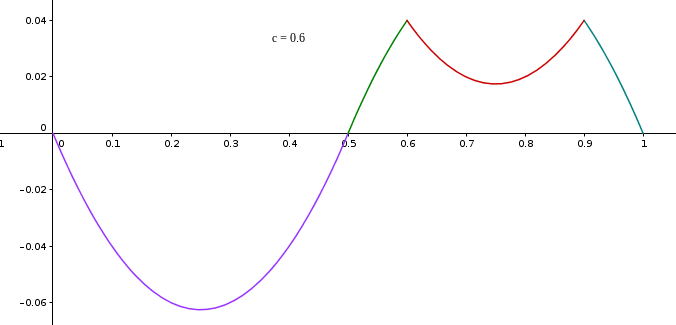
\includegraphics[scale=0.3]{exe2b}\quad
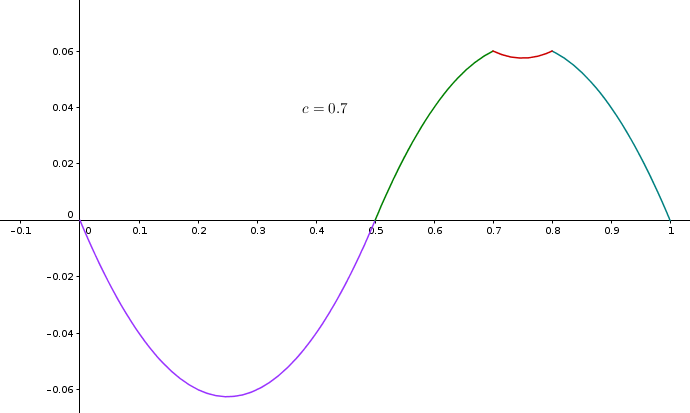
\includegraphics[scale=0.3]{exe2a}
\end{center}
\caption{The function $u_c$ as $c = 0.6$ and $c = 0.7$}
\end{figure}
\FloatBarrier


Now we will show that $u_c$ is a viscosity solution of $|Du_c(x)| = W(x)$ for any $c\in \left[\frac{1}{2},\frac{3}{4}\right]$. To do this, we only need to consider points in which $u_c$ is not smooth, that is $x = c$ and $x = \frac{3}{2} - c$. Also, we only need to consider $D^+u_c(x)$ since the set $D^-u_c(x)$ is always empty at non-smooth points of $u_c$. To begin with, we will give explicit formulas for $D^+u_c(c)$ and $D^+u_c\left(\frac{3}{2} - c\right)$.\\

\paragraph{\textbf{Case $x = c$.}} Recall that $p\in D^+u(c)$ iff $u(x) - u(c) \leq p(x-c)$
\begin{itemize}
\item Consider $x<c$, then it becomes
\begin{align*}
(x-c)\left(\frac{3}{2}-x-c\right) \leq p(x-c) \Longrightarrow \frac{3}{2}-x-c \geq p \Longrightarrow \frac{3}{2} - 2c\geq p.
\end{align*}
\item Consider $x>c$, then it becomes
\begin{align*}
(x-c)\left(x+c -\frac{3}{2}\right) \leq p(x-c) \Longrightarrow x+c -\frac{3}{2}\leq p \Longrightarrow 2c - \frac{3}{2}\leq p.
\end{align*}
\end{itemize}
Thus in this case we have
\begin{equation*}
p\in D^+u_c(c) \Longleftrightarrow |p|\leq \frac{3}{2}-2c.
\end{equation*}
Now we need to check that $|p|\leq W(c)$ for all $p\in D^+u_c(c)$, we have
\begin{equation*}
p\in D^+u_c(c) \Longrightarrow |p|\leq \frac{3}{2}-2c  = \frac{3-4c}{2} = W(c).
\end{equation*}
\vspace*{0.2cm}


\paragraph{\textbf{Case $x = \frac{3}{2}-c$.}}
Since $u_c$ and $W$ are symmetric through the line $x = \frac{3}{4}$, this case is completely similar to case $x= c$.
\end{itemize}
\end{proof}

%%%%%%% PROOF 2
\begin{proof}[\textbf{Proof 2}]
Consider the following equation
\begin{equation}\label{exer-HJ}
		\eps u^\eps(y) + H(y,Du^\eps)=0 \tag{HJ}.
\end{equation}
Plug the formula of $H$ into \eqref{exer-HJ} we have
\begin{equation*}
	 	\eps u^\eps(y)+ |Du^\eps(y)|-W(y)=0.
\end{equation*}
Observe that for each $\eps>0$, $u^\eps=0$ is a subsolution and $u^\eps=\frac{1}{\eps}$ is a supersolution. To see this, for $u^\eps=0$, let $\phi\in C^\infty$ s.t. $(\phi-u^\eps)(y_0)=0$ is a max. We have
$$D\phi(y_0)=Du^\eps(y_0)=0.$$
So $$\eps \phi(y_0) + H(y_0, D\phi(y_0))=0-W(y_0) \le 0.$$
Similarly, for $u^\eps=\frac{1}{\eps}$, let $\phi\in C^\infty$ s.t. $(\phi-u^\eps)(y_0)=0$ is a min. We have
$$\eps \phi(y_0) + H(y_0, D\phi(y_0))=1-W(y_0) \ge 0.$$
Therefore, if $v^\eps$ is a viscosity solution to \eqref{exer-HJ}, we have
	 $$1\ge \eps v^\eps \ge 0.$$
Thus, we have
\begin{equation}\label{exer-VanSonpt1}
	 	1\ge W(y) \ge |Dv^\eps(y)|.
\end{equation}
From here we conclude that $v^\eps$ is equi-Lipschitz with modulus 1. This is not enough to conclude anything about the convergence of $\eps v^\eps$ except of the result obtained in class. Luckily, we have more-- observe that
\begin{eqnarray*}
	 	\left|Dv^\eps\left(\frac{1}{4}\right)\right| \le W\left(\frac{1}{4}\right) =0,\\
	 	\left|Dv^\eps\left(\frac{3}{4}\right)\right| \le W\left(\frac{3}{4}\right) =0.
\end{eqnarray*}
So,
	 $$Dv^\eps\left(\frac{1}{4}\right)=Dv^\eps\left(\frac{3}{4}\right)=0.$$
That means, for all $\eps>0$, by plugging the above to our equation, $\eps v^\eps\left(\frac{1}{4}\right)=0,$ which means $v^\eps\left(\frac{1}{4}\right)=0$. Similarly, $v^\eps\left(\frac{3}{4}\right)=0$ for all $\eps>0$. Combine with \eqref{exer-VanSonpt1}, we deduce that for all $\eps>0$,
	 $$|v^\eps(y)| = \left|\int_{\frac{1}{4}}^y {v^\eps} '(t) dt\right| \le \int_{\frac{1}{4}}^y \left|{v^\eps} '(t)\right| dt \le \int_{\frac{1}{4}}^y 1 dt =\left|y-\frac{1}{4}\right|\le 1.$$
So, $\eps v^\eps(y)\to 0$ as $\eps\to 0$ and, therefore, $c=0$. The solutions to the problem are obtained similarly to proof 1.
\end{proof}
\vspace*{0.5cm}




\paragraph{\textbf{Exercise 4.}} Let $H\in \text{Lip}(\mathbb{R}^n\times \mathbb{R}^n)$ satisfying \vspace*{0.15cm}
\begin{itemize}
\item[(H1)] $\displaystyle \lim_{|p|\longrightarrow\infty} H(y,p) = +\infty$ uniformly in $y$,\vspace*{0.15cm}
\item[(H2)] $H(y+k,p) = H(y,p)$ for all $k\in \mathbb{Z}^n$\vspace*{0.15cm}.
\end{itemize}
Then $\overline{H}(p):\mathbb{R}^n\longrightarrow \mathbb{R}$ is a Lipschitz and coercive function.


\begin{proof}[\textbf{Proof 1.}] For $u\in C(\mathbb{T}^n)$ and $F:\mathbb{T}^n\times \mathbb{R}\times \mathbb{R}^n\longrightarrow \mathbb{R}$ is continous, we define
\begin{align*}
F(x,u(x),Du(x)) \leq C\;\text{in the viscous sense}\; &\Longleftrightarrow F(x,u(x),p) \leq C \qquad\forall\; p\in D^+u(x)\\
&\Longleftrightarrow u\;\text{is sub-solution of}\; F(x,u(x),Du(x)) = C,\\
F(x,u(x),Du(x)) \geq C\;\text{in the viscous sense}\; &\Longleftrightarrow F(x,u(x),p) \geq C \qquad\forall\; p\in D^-u(x)\\
&\Longleftrightarrow u\;\text{is super-solution of}\; F(x,u(x),Du(x)) = C.
\end{align*}
By assumption, there exists a constant $C>0$ such that
\begin{equation*}
|H(x,p) - H(x,q)|\leq C\Vert p-q\Vert\qquad\forall\;x,p,q\in \mathbb{R}^n.
\end{equation*}
We will prove the Lipschitz property of $\overline{H}$ by using the representation
\begin{equation}\label{nonconvex - representation of effective H}
\overline{H}(q) = \inf \left\lbrace c\in \mathbb{R}: \exists\;v\in C(\mathbb{T}^n): H(x,q+Dv(x))\leq c\;\text{in}\;\mathbb{T}^n\;\text{in viscous sense}\right\rbrace .
\end{equation}
\vspace*{0.2cm}
\paragraph{\textbf{Step 1.}} First of all, we prove that
\begin{equation}\label{sub - Lipschitz od effective H for p and 0}
\overline{H}(p) - \overline{H}(q) \leq C\Vert p - q\Vert.
\end{equation}
Let $u\in \text{Lip}(\mathbb{T}^n)$ is a periodic viscosity solution of the problem
\begin{equation}\label{Lipschitz E_q}
H(x,q + Du(x)) = \overline{H}(q)\tag{$E_q$}.
\end{equation}
By definition
\begin{align*}
\zeta\in D^+u(x) &\Longrightarrow H(x,q+\zeta) \leq  \overline{H}(q).
\end{align*}
%\delta\in D^-u(x) &\Longrightarrow H(x,\delta) \geq  \overline{H}(0)
We will show that
\begin{equation}\label{Lipschitz H(x,p+delta) leq C|p| + effective H(0) -- viscous sense}
H(x,p+Du(x)) \leq C\Vert p-q\Vert + \overline{H}(q)
\end{equation}
in the viscous sense. Indeed, for $\zeta\in D^+u(x)$, by the Lipschitz's property of $H$, we have
\begin{align*}
|H(x,p+\zeta) - H(x,q+\zeta)| \leq C\Vert p-q\Vert &\Longrightarrow
H(x,p+\zeta)\leq C\Vert p-q\Vert + H(x,q+\zeta)   \\
 &\Longrightarrow H(x,p+\zeta)\leq  C\Vert p-q\Vert + \overline{H}(q) \quad\quad \forall\; \zeta\in D^+u(x)\\
 &\Longrightarrow  H(x,p+Du(x)) \leq C\Vert p-q\Vert + \overline{H}(q) \quad\text{(vis-sense)}.
\end{align*}
Thus \eqref{Lipschitz H(x,p+delta) leq C|p| + effective H(0) -- viscous sense} is true, from the representation of $\overline{H}$ in \eqref{nonconvex - representation of effective H}, we obtain \eqref{sub - Lipschitz od effective H for p and 0} is true since
\begin{equation*}
\overline{H}(p) \leq C\Vert p-q\Vert + \overline{H}(q) \Longleftrightarrow \overline{H}(p) - \overline{H}(q) \leq C\Vert p-q\Vert.
\end{equation*}
%\item For $\delta\in D^-u(x)$, by the Lipschitz's property of $H$, we have
%\begin{align*}
%|H(x,p+\delta) - H(x,\delta)| \leq C\Vert p\Vert &\Longrightarrow
%H(x,\delta)\leq C\Vert p\Vert + H(x,p+\delta)   \\
% &\Longrightarrow \;\;\overline{H}(0)\;\;\, \leq  C\Vert p\Vert + H(x,p+\delta) \quad\quad \forall\; \delta\in D^-u(x)\\
% &\Longrightarrow \;\; \overline{H}(0)\;\;\, \leq C\Vert p\Vert + H(x,p+Du(x)) \quad\text{(vis-sense)}
%\end{align*}
\vspace*{0.2cm}

\paragraph{\textbf{Step 2.}} Similarly, doing quite similar to step 1, we obtain
\begin{equation}\label{super - Lipschitz od effective H for p and 0}
\overline{H}(q) - \overline{H}(p) \leq C\Vert p-q\Vert.
\end{equation}
From \eqref{sub - Lipschitz od effective H for p and 0} and \eqref{super - Lipschitz od effective H for p and 0} we obtain the Lipschitz's property of $\overline{H}$,
\begin{equation*}
|\overline{H}(p) - \overline{H}(q)|\leq C\Vert p-q\Vert.
\end{equation*}
\vspace*{0.2cm}

\paragraph{\textbf{Step 3.}} We now prove the coercivity of $\overline{H}$. First restate the coercivity of $H$ as
\begin{equation}\label{rewrite the uniformly in x coercivity of H}
\lim_{|p|\longrightarrow\infty} \left( \min_{x\in \mathbb{T}^n} H(x,p)\right) = +\infty.
\end{equation}
We start with a similar result as representation formula of $\overline{H}$ in \eqref{nonconvex - representation of effective H}, that is
\begin{equation}\label{nonconvex - representation of effective H - sup - inf}
\overline{H}(q) = \sup \left\lbrace c\in \mathbb{R}: \exists\;v\in C(\mathbb{T}^n): H(x,q+Dv(x))\geq c\;\text{in}\;\mathbb{T}^n\;\text{in viscous sense}\right\rbrace .
\end{equation}
Indeed, define
\begin{equation*}
\alpha = \sup \left\lbrace c\in \mathbb{R}: \exists\;v\in C(\mathbb{T}^n): H(x,q+Dv(x))\geq c\;\text{in}\;\mathbb{T}^n\;\text{in viscous sense}\right\rbrace .
\end{equation*}
Let $u\in C(\mathbb{T}^n)$ be the vicosity solution of the cell problem
\begin{equation*}
H(x,p+Du(x)) = \overline{H}(p) \qquad\text{in}\;\;\mathbb{T}^n.
\end{equation*}
Clearly, $\overline{H}(p)$ is admissible in the right hand of formula \eqref{nonconvex - representation of effective H - sup - inf}, thus $\overline{H}(p) \leq \alpha$. Now we want to prove $\alpha \leq \overline{H}(p)$, assume the contradiction, that is $\overline{H}(p) < \alpha$. Then there exists $(c,w)\in \mathbb{R}\times C(\mathbb{T}^n)$, $\overline{H}(p) < c \leq \alpha$ such that
\begin{equation*}
H(x,p+Dw(x)) \geq c >\overline{H}(p) = H(x,p+Du(x)).
\end{equation*}
Since $u,w$ are bounded, we can take $\varepsilon>0$ such that
\begin{equation*}
\varepsilon u(x) +H(x,p+Du(x)) < \frac{c+\overline{H}(p)}{2} < \varepsilon w(x) + H(x,p+Dw(x)).
\end{equation*}
By comparison principle, we have $u\leq w$ in $\mathbb{T}^n$, it's  a contradiction since we can always add a constant to make $w<u$.\\
Now using thus representation, let $\varphi = C\in  C^1(\mathbb{T}^n)$, and define
\begin{equation*}
c = \min_{x\in \mathbb{T}^n} H(x,p+D\varphi(x)) = \min_{x\in \mathbb{T}^n} H(x,p).
\end{equation*}
Then, $c$ is admissible in the formula of the representation \eqref{nonconvex - representation of effective H - sup - inf}, so that $\overline{H}(p)\geq c$, i.e
\begin{equation}\label{effective H(p) geq min x in Torus H(x,p)}
\overline{H}(p) \geq \min_{x\in \mathbb{T}^n} H(x,p).
\end{equation}
Now combine \eqref{effective H(p) geq min x in Torus H(x,p)} with \eqref{rewrite the uniformly in x coercivity of H} we obtain
\begin{equation*}
\lim_{|p|\longrightarrow \infty} \overline{H}(p) \geq \lim_{|p|\longrightarrow \infty} \left( \min_{x\in \mathbb{T}^n} H(x,p) \right) = +\infty.
\end{equation*}
Thus $p\longmapsto \overline{H}(p)$ is coercive and the proof is complete.
\end{proof}

%%%%%PROOF 2
\begin{proof}[\textbf{Proof 2}] Lipschitz part.\\
Let $p, q\in \R^n$, we want to show that $|\bar{H}(p)-\bar{H}(q)|\le C|p-q|$. Let $u^\eps$ and $v^\eps$ be solutions to the following problems
\begin{equation}
		\eps u^\eps + H(x, Du^\eps + p)=0
\end{equation}
	and
\begin{equation}
		\eps v^\eps + H(x, Dv^\eps + q)=0.
\end{equation}
We have, by ``Lipschitzivity'',
	$$|H(x, Du^\eps + p) - H(x, Du^\eps + q)| \le C|p-q|.$$
Thus,
	$$|-\eps u^\eps - H(x, Du^\eps + q)| \le C|p-q|,$$
which implies
	\begin{equation}
	 \eps u^\eps+C|p-q| + H(x, Du^\eps +q) \ge 0. \label{inequality_1}
	\end{equation}
	Thus, $u^\eps + \frac{C|p-q|}{\eps}$ is a supersolution to (29) and
	$$u^\eps + \frac{C|p-q|}{\eps}\ge v^\eps,$$
	meaning $$\eps v^\eps-\eps u^\eps \le C|p-q|.$$

	Similarly, we obtain
	$$-C|p-q| \le \eps v^\eps-\eps u^\eps .$$
	Thus, $|\eps u^\eps - \eps v^\eps| \le C|p-q|$. Let $\{ \eps_j\}$ be a sequence such that $\eps_j u^{\eps_j} \to \bar{H}(p)$ and $\eps_j v^{\eps_j} \to \bar{H}(q)$, we then have
	$$|\bar{H}(p)- \bar{H}(q)| \le C|p-q|.$$

	Coercivity part:

	Let $M>0$. Pick $|p|$ big enough so that $H(x,p)>M$.

	Let $u$ be the solution to the cell problem
	$$H(x, Du+p) = \bar{H}(p).$$
	Since $u$ is continuous and periodic, $u$ has a max at $x_0$. So consider the test function $\phi(x)={u(x_0)}$. We have that, by definition of viscosity solution,
	$$M< H(x,D\phi(x_0)+p)=H(x,p) \le \bar{H}(p).$$
\end{proof}

\vspace*{0.2cm}




\paragraph{\textbf{Exercise 5}.} Let $H\in \text{Lip}(\mathbb{R}^n\times \mathbb{R}^n)$ satisfying\vspace*{0.15cm}
\begin{itemize}
\item[(H1)] $\displaystyle \lim_{|p|\longrightarrow\infty} H(y,p) = +\infty$ uniformly in $y$,\vspace*{0.15cm}
\item[(H2)] $H(y+k,p) = H(y,p)$ for all $k\in \mathbb{Z}^n$\vspace*{0.15cm}.
\end{itemize}
Assume $p\longrightarrow H(y,p)$ is convex for any $y\in \mathbb{T}^n$, then $p\longmapsto\overline{H}(p)$ is also convex.

\vspace*{0.2cm}

\begin{proof}[\textbf{Proof 1.}]
%For $u\in C(\mathbb{T}^n)$ and $F:\mathbb{T}^n\times \mathbb{R}\times \mathbb{R}^n\longrightarrow \mathbb{R}$ is continous, we define
%\begin{align*}
%F(x,u(x),Du(x)) \leq C\;\text{in the viscous sense}\; &\Longleftrightarrow F(x,u(x),p) \leq C \qquad\forall\; p\in D^+u(x)\\
%&\Longleftrightarrow u\;\text{is sub-solution of}\; F(x,u(x),Du(x)) = C\\
%F(x,u(x),Du(x)) \geq C\;\text{in the viscous sense}\; &\Longleftrightarrow F(x,u(x),p) \geq C \qquad\forall\; p\in D^-u(x)\\
%&\Longleftrightarrow u\;\text{is super-solution of}\; F(x,u(x),Du(x)) = C
%\end{align*}
We will prove the convexity of $p\longmapsto\overline{H}(p)$ by the representation formula of $\overline{H}$, that is
\begin{align*}
\overline{H}(q) &= \inf \left\lbrace c\in \mathbb{R}: \exists\;v\in C(\mathbb{T}^n): H(x,q+Dv(x))\leq c\;\text{in}\;\mathbb{T}^n\;\text{in viscous sense}\right\rbrace \\
	            &= \inf\left\lbrace \sup_{x\in \mathbb{T}^n} H(x,q+D\varphi(x))\;\;:\varphi\in C^1(\mathbb{T}^n)\right\rbrace.
\end{align*}
Let $u\in\;\text{Lip}(\mathbb{T}^n)$ is a viscosity solution of the problem
\begin{equation}\label{Epp}
H(x,p+Du(x)) = \overline{H}(p) \tag{$E_p$}.
\end{equation}
Let $\varphi\in C^1(\mathbb{T}^n)$ arbitrary and let
\begin{equation*}
C = \max_{x\in \mathbb{R}^n} H(x,q+D\varphi(x)).
\end{equation*}
For $\lambda\in (0,1)$, consider the function
\begin{equation*}
w = \lambda u + (1-\lambda) \varphi.
\end{equation*}
We will show that (in the viscous sense)
\begin{equation}\label{Elambda p + 1-lambda q}
H\left(x,\lambda p +(1-\lambda)q+ Dw\right) \leq \lambda \overline{H}(p) + (1-\lambda)C .
\end{equation}
To do this, we need to show that for any $\zeta\in D^+w(x)$, then
\begin{equation*}
H\left(x,\lambda p +(1-\lambda)q+ \zeta\right) \leq \lambda \overline{H}(p) + (1-\lambda)C.
\end{equation*}
\vspace*{0.1cm}
\paragraph{\textbf{Lemma.}} \textit{Let $u\in C(\Omega)$, then
\begin{equation*}
D^+w(x) = \lambda D^+u(x) + (1-\lambda)D\varphi(x)
\end{equation*}
for any $\varphi\in C^1(\Omega)$, $w = \lambda u + (1-\lambda)\varphi$ and $\lambda\in [0,1]$.}\\
\vspace*{0.3cm}
\begin{proof}[\textbf{Proof of lemma}] It's easy to see that $\lambda D^+u(x) + (1-\lambda)D\varphi(x) \subseteq D^+w(x)$. For the converse, let $\zeta\in D^+u(x)$, setting $\alpha = \zeta - (1-\lambda)D\varphi(x)$, then
\begin{align*}
\frac{\lambda u(y) - \lambda u(x) - \langle \alpha,y-x \rangle}{\Vert y-x\Vert} = &\frac{w(y) - w(x) - \langle \zeta,y-x \rangle}{\Vert y-x\Vert} \\
- &(1-\lambda)\frac{\varphi(y) - \varphi(x) - \langle D\varphi(x),y-x\rangle}{\Vert y-x\Vert}.
\end{align*}
Taking $\limsup$ of both sides, we have $\alpha\in D^+(\lambda u)(x)$, therefore $\frac{\alpha}{\lambda}\in D^+u(x)$, then
\begin{equation*}
\delta = \lambda\left( \frac{\alpha}{\lambda}\right) + (1-\lambda)D\varphi(x) \subseteq \lambda D^+u(x) + (1-\lambda)D\varphi(x).
\end{equation*}
The proof of lemma is complete.
\end{proof}
\vspace*{0.2cm}
By above lemma, there exists $\alpha\in D^+u(x)$ such that $\zeta = \lambda \alpha + (1-\lambda)D\varphi(x)$, using the convexity in $p$ of $H$ we obtain
\begin{align*}
H\left(x,\lambda p +(1-\lambda)q + \zeta\right) &= H\left(x,\lambda p +(1-\lambda)q + \lambda \alpha + (1-\lambda)D\varphi(x)\right) \\
&\leq \lambda H(x,p+\alpha) + (1-\lambda)H(x,q+D\varphi) \\
&\leq \lambda \overline{H}(p) + (1-\lambda)C.
\end{align*}
Thus in sense of viscosity, we obtain \eqref{Elambda p + 1-lambda q} is true. By representation formula for $\overline{H}\left(\lambda p + (1-\lambda)q\right)$ we have
\begin{equation*}
\overline{H}\left(\lambda p + (1-\lambda)q\right) \leq \lambda \overline{H}(p) + (1-\lambda)C.
\end{equation*}
In other words, we have
\begin{equation*}
\overline{H}\left(\lambda p + (1-\lambda)q\right) - \lambda \overline{H}(p) \leq  (1-\lambda)C = (1-\lambda)\max_{x\in \mathbb{T}^n} H(x,q+D\varphi(x))
\end{equation*}
and since $\varphi\in C^1(\mathbb{T}^n)$ is arbitrary, we get
\begin{equation*}
\overline{H}\left(\lambda p + (1-\lambda)q\right) - \lambda \overline{H}(p)  \leq  (1-\lambda) \inf_{\varphi\in C^1(\mathbb{T}^n)} \max_{x\in \mathbb{T}^n} H(x,q+D\varphi(x)) = (1-\lambda)\overline{H}(q).
\end{equation*}
Thus,
\begin{equation*}
\overline{H}\left(\lambda p + (1-\lambda)q\right)  \leq \lambda \overline{H}(q) + (1-\lambda)\overline{H}(q)
\end{equation*}
and $\overline{H}$ is convex.
\end{proof}

%%%%PROOF 2
\begin{proof}[\textbf{Proof 2}]
Suppose $\bar{H}(p)$ is not convex.  There are $p$, $q$ such that
	\begin{equation}
		\bar{H}((1-k)p + kq) > (1-k)\bar{H}(p)+k\bar{H}(q)
	\end{equation}
	for some $k\in (0,1)$. Let $u$ be a solution of
	\begin{equation}
		H(x, Du + (1-k)p + kq) = \bar{H}((1-k)p + kq)
	\end{equation}
	and $v_p, v_q$ be solutions of
	$$H(x,Dv + p)= \bar{H}(p)$$
	and $$H(x,Dv + q)= \bar{H}(q)$$
	respectively.
	(32) Implies that
	\begin{eqnarray*}
		\bar{H}((1-k)p + kq)	&>& 	(1-k)H(x,Dv_p + p)+ kH(x,Dv_q + q)\\
						&\ge&	H(x, (1-k)(Dv_p + p) + k(Dv_q +q)) \\
						&=&		H(x, (1-k)Dv_p+ kDv_q + (1-k)p +kq).
	\end{eqnarray*}
	So, $(1-k)v_p + kv_q$ is a subsolution to (33). Therefore, $u \ge (1-k)v_p + kv_q$. But if $u$ is a solution to (33), $u+C$ is also a solution to (33), which makes
	$$ u + C \ge (1-k)v_p + kv_q$$ for all $C$, which is a contradiction since $v_p$ and $v_q$ are real-valued functions.
\end{proof}

\nocite{*}
\bibliographystyle{plain}
\bibliography{bib}



\end{document}
